\chapter{Hidráulica Aplicada}
\section{Introducción}
\subsection{Ecuaciones básicas}
Considerando el teorema del transporte de Reynolds
\begin{equation}
    \frac{dN}{dt}_{system} = \frac{\partial}{\partial t} \int_{CV} \eta \rho 
\end{equation}


Ecuación de energía:

Ecuación de continuidad:
\begin{align*}
    &m_1 - m_2 =\frac{\Delta m}{t}\\
    &m = \frac{m}{t}\; \rho = \frac{m}{V}\\
    &m =\rho V
\end{align*}
Entonces si el flujo es permanente:
\begin{equation}
    m_1 - m_2 = 0
\end{equation}

Ecuación de energía (Ecuación de Bernoulli para fluido real)
\begin{equation}
    z_1 + \frac{p_1}{\gamma} +\frac{v_1^2}{2g} + H_{T.B} = z_2 + \frac{p_2}{\gamma} +\frac{v_2^2}{2g} +\sum h_r
\end{equation}
Ecuación de cantidad de movimiento (Segunda ley de Newton)
\begin{equation}
    \sum F =\sum \rho Q \bar{v}
\end{equation}
Métodos experimentales para solución de problemas:

\begin{enumerate}
    \item \textbf{Análisis dimensional:} El análisis dimensional es una herramienta conceptual muy utilizada en la física, la química y la ingeniería para ganar comprensión de fenómenos que involucran una combinación de diferentes cantidades físicas. Es además. rutinariamente utilizada para verificar relaciones y cálculos, así como para construir hipótesis razonables sobre situaciones complejas, que puedan ser verificadas experimentalmente.
    \item \textbf{Dimensión:} La propiedad de una variable, por ejemplo el sistema [MLT]: Longitud-Masa-tiempo ó [FLT]: Fuerza-Longitud-Tiempo 
\end{enumerate}

\begin{definition}[Unidad]
    Es una magnitud arbitraria de una dimensión empleada como estádar para propósitos de medición o cálculo (Metro, kilográmo, segundo, etc.)
\end{definition}

Todas las ecuaciones que relacionan cantidades físicas deberán ser homogéneas o sea que los términos de un lado de la ecuación deberán ser igual a los del otro, en operaciones matemáticas como diferenciación e integración la homogeneidad dimensional no afecta. En ingenería se usa frecuentemente en la verificación de las fórmulas comprobando que las unidades de los dos lados de la ecuación sean iguales.

Cada variable además de tener un valor numérico, tiene una dimensión, osea una combinación de unidades de referencia. Si la variable se conserva constante, se llama parámetro

\begin{example}
    Velocidad: $V,\left[M^0L^1T^{-1}\right]$, $\left[\frac{L}{T}\right]$
\end{example}

\begin{theorem}[Homogeneidad]
    Toda ecuación para que sea válida, será dimensionalmente homogénea
\end{theorem}

\begin{example}
    Para un flujo que está pasando en un orificio, se desea conocer la velocidad con que pasa el fluido, considerando que el fluido sea agua, utilizando técnica adimensional, obtener la expresión para velocidad
\end{example}
\begin{figure}[h!]
\centering
  \includegraphics[width=0.5\textwidth]{ha1.pdf}
  \caption{Flujo de agua a través de un orificio}
  \label{ha1}
\end{figure}

\textit{ Sol. }

De la carga sobre el orificio $H$ la unidad es $[L]$, del eso del fluido, como es en cantidad cinemática no depende de otra más que la gravedad $g$, así que $[LT^{-2}]$, Densidad $\rho$, de la viscodidad $\mu$, tensión superficial $\sigma$ del módulo de elasticidad $K$, en sólidos se usa comúnmente $E$, entonces se busca la expresión o relación funcional que nos da la información requerida. $f(V,H,G,\rho,\mu,\sigma,K\dots)=0$ a ésto se le llama función de variables o relación funcional, de aquí se seleccionan las que más intervienen en el problema para resolver el problema, para este caso consideramos la más importantes para éste flujo a la carga $H$, y a la gravedad las otras no tienen efecto significativo, se reduce a sólo $f(V,H,g)=0$

Obtenga un producto adimensional: $\pi=V^{x_1}H^{x_2}g^{x_4}$ como es un producto adimensional, debe tener dimensiones cero: $\pi^0=V^{x_1}H^{x_2}g^{x_3}=\left[MLT\right]^0=\left[L/T\right]^{x_1}\left[L\right]^{x_2}\left[L/T^2\right]^{x_3}$ de manera que se simplifica hsta llegar a $\pi^0=\left[M^0L^0T^0\right]$ para cumplir con la igualdad de los exponentes en cada variable deben ser iguales, entonces: 
\begin{align*}
    &\text{Para M, }\quad 0x_1+ 0x_2+ 0x_3 =0\\
    &\text{Para L, }\quad x_1+ x_2+ x_3 = 0\\
    &\text{Para T, }\quad -x_1+ 0x_2 - 2x_3 =0
\end{align*}
Se ve reducido a
\begin{equation*}
    \begin{cases}
        &x_1 +x_2 + x_3= 0\\
        &- x_1 - 2x_3= 0
    \end{cases}
\end{equation*}
Un sistema con más incógnitas que ecuaciones, que tiene solución infinita, como buscamos la velocidad $V$, lo ponemos con exponente $x_1=1$ con lo que obtenemos $x_2=-1/2$ y $x_3=-1/2$, sustituyendo en el producto adimensional: $\pi=V^1H^{-1/2}g^{-1/2}$ así que $V\pi H^{-1/2}g^{-1/2}$, $V=C \sqrt{gH}$: Ecuación de Torricelli. Para obtener la ecuación real con valores observados y con la ecuación ajustada de la gráfica con $C=\pi$ que se ha estudiado como: $V=C \sqrt{gH}$ donde $C=C_v \sqrt{2gH}$, $C=C_d\sqrt{2g}$ y $C_d=C_cC_v$

\subsubsection{Matriz de exponentes}
Es una matriz donde se colocan en un renglón las variables que intervienen en un problema y en una colúmna sus dimensiones, escribiendo en el crice respectivo el exponente de la unidad correspondiente.
\begin{example}
    Las dimensiones que intervienen en el problema $f(V,H,g)=0$ son: $\left[M^0L^1T^{-1}\right]^{x_2}\left[M^0L^1T^{-2}\right]^{x_1}=\left[M^0L^0T^0\right]$
\end{example}
\textit{ Sol. }
\begin{table}[h!]
    \centering
    \begin{tabular}{@{}cccc@{}}
    \toprule
      & V  & H & g  \\ \midrule
    M & 0  & 0 & 0  \\
    L & 1  & 1 & 1  \\
    T & -1 & 0 & -2 \\ \bottomrule
    \end{tabular}
    \caption{Matriz de exponentes}
    \label{tabha1}
\end{table}

Entonces:
\begin{align*}
    &\text{Para M, }\quad 0x_1+ 0x_2+ 0x_3 =0\\
    &\text{Para L, }\quad x_1+ x_2+ x_3 = 0\\
    &\text{Para T, }\quad -x_1+ 0x_2 - 2x_3 =0
\end{align*}
Así como en el ejemplo anterior, el sistema fue creado para obtener la velocidad, se asigna el valor de 1. Además de satisfacer la igualdad numérica se tiene que:
\begin{enumerate}
    \item Ser dimensionalmente homogénea
    \item La ecuación sólo es válida para cierto rango de variables
    \item No se pueden hacer todas las operaciones matemáticas con ella
    \item Para poder hacer la operación es conveniente hacer adimensionales las variables
\end{enumerate}

En experimentación las variables se clasifican en dos tipos: dependeintes e independietnes - La primera es la que interesa determinar la velocidad o presión. La segunda representan propiedades del fluido como densidad y viscosidad

\begin{table}[h!]
    \centering
    \begin{tabular}{@{}cccccccc@{}}
    \toprule
                             & M  & L  & T  &  & F  & L  & T  \\ \midrule
    \textbf{Masa}            & 1  & 0  & 0  &  & 1  & -1 & 2  \\
    Longitud                 & 0  & 1  & 0  &  & 0  & 1  & 0  \\
    Tiempo                   & 0  & 0  & 1  &  & 0  & 0  & 1  \\
                             &    &    &    &  &    &    &    \\
    \textbf{Área}            & 0  & 2  & 0  &  & 0  & 2  & 0  \\
    Volumen                  & 0  & 3  & 0  &  & 0  & 3  & 0  \\
    Ángulo                   & 0  & 0  & 0  &  & 0  & 0  & 0  \\
                             &    &    &    &  &    &    &    \\
    Frecuencia               & 0  & 0  & -1 &  & 0  & 0  & -1 \\
    Velocidad                & 0  & 1  & -1 &  & 0  & 1  & -1 \\
    Aceleración              & 0  & 1  & -2 &  & 0  & 1  & -2 \\
    Gasto                    & 0  & 3  & -1 &  & 0  & 3  & -1 \\
    Circulación              & 0  & 2  & -1 &  & 0  & 2  & -1 \\
    Densidad                 & 1  & -3 & 0  &  & 1  & -4 & 2  \\
                             &    &    &    &  &    &    &    \\
    \textbf{Peso específico} & 1  & -2 & -2 &  & 1  & -3 & 0  \\
    Viscosidad dinámica      & 1  & -1 & -1 &  & 1  & -3 & 1  \\
    Viscosidad cinemática    & 0  & 2  & -1 &  & 0  & 2  & -1 \\
    Tensión superficial      & 1  & 0  & -2 &  & 1  & -1 & 0  \\
    Módulo de elasticidad    & 1  & -1 & -2 &  & 1  & -2 & 0  \\
    Compresibilidad          & -1 & 1  & 2  &  & -1 & 2  & 0  \\
                             &    &    &    &  &    &    &    \\
    Fuerza                   & 1  & 1  & -2 &  & 1  & 0  & 0  \\
    Presión                  & 1  & -1 & -2 &  & 1  & -2 & 0  \\
    Par                      & 1  & 2  & -2 &  & 1  & 1  & 0  \\
    Energía trabajo          & 1  & 2  & -2 &  & 1  & 1  & 0  \\
    Potencia                 & 1  & 2  & -3 &  & 1  & 1  & -1 \\
    Cantidad de movimiento   & 1  & 1  & -1 &  & 1  & 0  & 1  \\
    Impulso                  & 1  & 1  & -1 &  & 1  & 0  & 1  \\ \bottomrule
    \end{tabular}
    \caption{Variables más comunes y sus dimensiones}
    \label{tabha2}
\end{table}
\begin{theorem}[De Buckingham-Vaschy]
    Sea la función $f\left(x_1,x_2,x_3\dots x_m\right)=0$
    Función que relaciona $m$ variables y $r$ es el rango de la matriz de exponentes de las variables. Existe otra función $f\left(\pi_1,\pi_2,\pi_3\dots\pi_{m-r}\right)=0$ con la ventaja de simplificar grandemente al problema y también da información útil acerca del comportamiento del fenómeno.
\end{theorem}

Para hacer esta simplificación
\begin{itemize}
    \item Formar la matriz de exponentes y se determina su rango
    \item Se construye de ecuaciones utilizando como coeficientes elementos de la matriz
    \item Se encuentra $m-r$ soluciones a éste soluciones para obtener un producto adimensional.
\end{itemize}

\begin{example}
    Obtener la ecuación para gastos través de un tubo capilar horizontal el cual depende de la caída de presión por unidad de longitud $\frac{\Delta p}{l}$ del diámetro del tubo $D$ y la viscosidad del fluido $\mu$ mediante la técnica de análisis dimensional
\end{example}

\textit{ Sol. }

Relación funcional: $f\left(Q,\frac{\delta p}{l},D,\mu\right)=0$
\begin{table}[h!]
    \centering
    \begin{tabular}{@{}ccccc@{}}
    \toprule
      & $Q$ & $\frac{\Delta p}{l}$ & $D$ & $\mu$ \\ \midrule
    M & 0   & 1                   & 0   & 1     \\
    L & 3   & -2                  & 1   & -1    \\
    T & -1  & -2                  & 0   & -1    \\ \bottomrule
    \end{tabular}
    \caption{Matriz de exponentes}
    \label{tabha3}
\end{table}

Rango de la matriz de exponentes $r=3$, del teorema $\pi$ o de Buckingham $m-r=4-3=1$

De la diferencia de presión sobre longitud, se tiene:
\begin{equation*}
    \frac{\frac{N}{m^2}}{m} = \frac{kg\cdot \frac{m}{s^2}}{m^2} = \frac{\frac{m\cdot \frac{L}{T^2}}{L^2}}{L} = \frac{MLT^{ - 2}}{L^3} = \frac{MT^{ - 2}}{L^2}
\end{equation*}
Siguiendo los mismos pasos, se llega a la matriz de exponentes.

Se reduce a $f(\pi)=0$, así que sólo hay que encontrar un producto adimensional $\pi= Q^{x_1}\frac{\Delta p^{x_2}}{l}D^{x_3}\mu^{x_4}$
\begin{align*}
    &\text{Para M, }\quad 0x_1+ 0x_2+ 0x_3 + x_4 =0\\
    &\text{Para L, }\quad 3x_1 - 2x_2+ x_3 - x_4 = 0\\
    &\text{Para T, }\quad -x_1 - 2x_2 + 0x_3 - x_4 =0
\end{align*}
Aplicando la primera recomendación o regla se resuelve el sistema $x_2=-1,x_3=-4,x_4=1,x_1=1$ así mismo $\pi= Q^1\frac{\Delta p^{-1}}{l}D^{-4}\mu^1$ así se llega a la ecuación solicitada
\begin{equation*}
    Q = c\frac{\Delta pD^4}{\mu l}
\end{equation*}

Ecuación de Poiseuille
\begin{equation}
    Q = \frac{\pi \Delta Pr^4}{8\eta L}
\end{equation}
Donde $Q$ es el flujo, $r$ el radio del vaso, $\Delta P$ el gradiente de presión, $\eta$ la viscosidad y $L$ la longitud del vaso

\textbf{Recomendaciones para formar productos adimensionales}

\textbf{REGLA 1.} Hacer que la variable dependiente aparezca en el numerador de un solo producto adimensional, de preferencia con el exponente 1 y no aparezca en ningún otro producto con excepción importante de la velocidad.

\textbf{REGLA 2.} Tratar de formar productos adimensionales ya conocidos o estándar como por ejemplo Reynolds, Froude, etc.

\textbf{REGLA 3.} Las variables que describen la geometria del problema y cuya dimensión es una longitud, se pueden hacer adimensionales simplemente seleccionando una longitud como caracteristica y dividiendo cada variable entre esa longitud, ejemplo, longitud como característica y dividiendo cada variable entre esa longitud, ejemplo, sea L,X,Y entonces los productos serán: $T_1= X/L$, $T_2= Y/L$.

En los casos que después de aplicar los tres criterios anteriores aún queden productos por determinar, será necesario asignar valores a las otras incógnitas para obtener las soluciones faltantes
\begin{itemize}
    \item Las variables que representan las propiedades del fluido exceptuando la densidad, como viscosidad, módulo de elasticidad, tensión superficial, etc. Deben de aparecer solas en un solo producto adimensional.
    \item Hay que buscar productos no solo correctos sino también que satisfagan criterios de sencillez y naturalidad
    \item No deben aparecer demasiadas variables en un producto adimensional, (generalmente intervienen 3 o 4 aunque algunos casos mas de 4) 
    \item En los productos adimensionales deben de estar todas las variables que aparecen en el problema (si falta alguna obviamente la solución es incorrecta) y que los productos sean independientes 
\end{itemize}
Por lo tanto cuando se usan variables repetitiva usualmente se selecciona a la velocidad, a la densidad y una longitud caracteristica, sin olvidarse las recomendaciones anteriores

Desventajas de usar el análisis dimensional

\begin{itemize}
    \item Reduce el número de variables, pero puede complicar la expresión entre si. 
    \item Pueden aparecer nuevas variables sin interés para el problema pero que por necesidades dimensionales es necesario incluir por ejemplo la gravedad
    \item A pesar de que las variables involucradas están comprendidas en un rango finito de valores, al utilizar productos adimensionales estos pueden tener alores infinitos
    \item Las variables repetitivas en los productos adimensionales originan correlaciones espurias
\end{itemize}
\subsection{Semejanza en los modelos hidráulicos}
Cuando en un análisis analítico las hipótesis planteadas para simplificar las soluciones además de restar generalidad, puede llegar a falsear los resultados a tal grado que no tengan relación alguna con el comportamiento real del fenómeno y en ocasiones resulta difícil establecer condiciones fronteras previas a cualquier solución matemática y se ve supeditadas a la experimentación.

Los modelos hidráulicos han encontrado creciente aplicación para controlar y modificar diseños analíticos de estructuras hidráulicas, es posible experimentar a costos relativamente bajos y con economías sustanciales de tiempo hasta obtener condiciones óptimas.

Basado en la teoría de \texttt{Kline} donde: \emph{``Si dos sistemas obedecen al mismo grupo de ecuaciones y condiciones gobernantes y si los valores de todos los parámetros y las condiciones se hacen idénticas, los dos sistemas deben de exhibir comportamientos similares con tal de que exista una solución única para el grupo de ecuaciones y condiciones''}

Por lo tanto, la similitud o semejanza va más allá de los aspectos superficiales de similitud geométrica, la similitud geométrica raramente es perfecta debido a que es imposible satisfacer todas las condiciones requeridas para lograrla , va a depender del modelo, de las mediciones que haga el operador, precisión del instrumental que se utiliza, exactitud con que se construye el modelo, los efectos de escala y reconocer que no existe similitud absoluta, sino mas bien, similitudes imperfectas cuyo fin será predecir el comportamiento del prototipo a través de los resultados  obtenidos experimentalmente en el modelo, es necesario en hidráulica que existan las similitudes siguientes

\begin{itemize}
    \item Geométrica (escala de líneas)
    \item Cinemática (velocidad y aceleración)
    \item Dinámica (fuerzas)
\end{itemize}
Aunque no son loas únicas , también se pueden considerar para casos no
isotérmicos y químicos a:
\begin{itemize}
    \item Térmica (temperatura)
    \item Química (Concentraciones)
\end{itemize}
\subsubsection{Similutud geométrica}
Modelo a escala no distorsionado en sus líneas: $Le_v=Le_h$

Para que exista similitud geométrica entre modelo y prototipo, debe cumplirse que
todas las relaciones de todas las dimensiones lineales homólogas sean
constantes.
\begin{equation}
    \text{Escala}=\frac{\text{Magnitud cualquiera en el prototipo}}{\text{Magnitud homóloga en el modelo}}
\end{equation}

Las magnitudes homólogas son aquellas que se corresponden, a una en el modelo y otra en prototipo, esto es, si ciertas dimensiones del prototipo y modelo se seleccionan y se designa $Lp$ al prototipo y $Lm$ al modelo, la similitud geométrica significa

$Le=$ Escala de líneas constante, $Le=\frac{L_p}{L_m}$, $L_p=$ longitud en el prototipo (Estructura real), $L_m=$ longitud en el modelo.
\begin{equation}
    Le = \frac{H_p}{H_m} = \frac{B_p}{B_m}\quad \text{Escala natural no distorsionada}
\end{equation}

En casos donde se tienen ríos o estructuras con tirantes pequeños y es necesario
distorsionar los modelos, teniendo modelos distorsionados en sus líneas 

También debe tenerse en cuenta las rugosidades de modo que la relación de
pérdidas sea la misma

\subsubsection{Similiutd cinemática}
Existe semejanza cinemática, si la relación entre la magnitud de cualquier
velocidad; Escala de velocidades y aceleración $Ve= \frac{v_p}{v_m}$ la similitud existe si $v_e=$constante $a_e=\frac{a_p}{a_m}$ constante, para cada punto homólogo.
Punto homologo, es aquel que se corresponde con otro

\subsubsection{Similitud dinámica}
Escala de Fuerzas $F_e=\frac{F_p}{F_m}m_ea_e$  similitud existe si $F_e=constante$ e en todos sus puntos homólogos

Las fuerzas que intervienen comúnmente en fluidos son:
\begin{itemize}
    \item Fuerzas de presión
    \item Número de Euler $E=\frac{\text{inercia}}{\text{presión}}$
    \item Fuerzas de peso propio
    \item Número de Froude $Fr=\frac{\text{inercia}}{\text{gravedad}}$
    \item Fuerzas viscosas
    \item Número de Reynolds $Re=\frac{\text{inercia}}{\text{viscosas}}$ 
    \item Fuerzas Elásticas
    \item Número de Mach $M=\frac{\text{inercia}}{\text{elásticas}}$
    \item Fuerzas de tensión superficial
    \item Número de Weber $W=\frac{\text{inercia}}{\text{tensión superficial}}$
\end{itemize}

Modelo a escala distorsionado en sus líneas
$Le_v \neq Le_h$
Se emplean cuando no se puede medir con precisión valores de tirante, velocidad, etc. por tener dimensiones
no fáciles de escalar

\begin{example}
    un río con un tramo de 2,000m de longitud $L_h$ y un tirante máximo de 4 metros $L_v=y_p$
\end{example}

\textit{ Sol. }

Si dispone de un laboratorio con una longitud máxima de 30 metros, suponemos un $Le = 70 = \frac{L_p}{L_m}$,
$L_p = 2000 m$, $Lm = \frac{2000}{30} = 28.57m$, $y_m = \frac{4}{70} = 0.057m$
No útil para fines prácticos medir tirantes, se distorsiona, entonces:
\begin{align*}
    &Le_v = 20&&Le_h = 70\\
    &y_m = \frac{4}{20}= 0& 0.2m&L_m = \frac{200}{30} = 28.57m
\end{align*}

\subsubsection{Ley de Froude}
Cuando los efectos más importantes en el movimiento del flujo son los de la gravedad
Ley de similitud Froude se cumple cuando $Fr_p=Fr_m$ ó $\frac{Fr_p}{Fr_m}=1$
\begin{align*}
    &\frac{V_p}{\sqrt{g_pl_p}} \frac{V_m}{\sqrt{g_pl_m}}\\ 
    &Ve = \frac{v_p}{v_m} =\frac{\sqrt{g_pl_p}}{g_ml_m} =\left(g_eL_e\right)^{\frac{1}{2}}\\ 
    &V_p =\left(g_eL_e\right)^{\frac{1}{2}}V_m\\
    &Q_e= A_cV_e = L_eL_eV_e =\left(L_e\right)^2 = g_e^{\frac{1}{2}}L_e^{\frac{5}{2}} = \frac{Q_p}{Q_m}
\end{align*}

\begin{example}
    Se utiliza un modelo a escala 1:49 de una presa para predecir las condiciones de flujo en el prototipo. Si el gasto de diseño es de $15,000 m^3/s$, ¿que velocidad de flujo debe de establecerse en el modelo para simular esta condición si se mide una velocidad de 2 m/s en un punto en el modelo?, ¿cual sería el gasto en el modelo?
\end{example}

\textit{ Sol. }

El efecto del movimiento del agua, más importante es la gravedad, por lo tanto, se aplica la ley Froude

Datos $Le=49$, $Q_p = 15,000 m^3/s$, $V_m = 2m/s$, Incógnitas, $Vp=?$, $Qm=?$

\begin{align*}
    &Ve =\left(Le\right)^{\frac{1}{2}} = 48^{0.5} = 7\\
    &Ve = \frac{v_p}{v_m} \implies v_p = 7\cdot 2\frac{m}{s} = 4\frac{m}{s}\\
    &Qe = ge^{\frac{1}{2}} = \frac{Q_p}{Q_m};\quad Qe = Le^{\frac{5}{2}};\quad Q_m = \frac{Q_p}{Le^{\frac{5}{2}}} = \frac{15,000}{16,807} = 0.892 \frac{m^3}{s}
\end{align*}

\subsubsection{Ley de Reynolds}

Cuando los efectos más importantes en el movimiento del flujo son los de los efectos viscosos, la ley de similitud Reynolds se cumple cuando $Re_p=Re_m$ ó $\frac{Re_p}{Re_m}=1$.
\begin{align*}
    &Ve = \frac{v_p}{v_m} =\frac{\frac{V_p\cdot l_p}{\frac{\mu p}{\rho p}}}{\frac{V_m\cdot l_m}{\frac{\mu m}{\rho m}}} =\mathcal{V}L_e^{ 1}\\
    &Qe = L_e^2\cdot V_e\implies L_e^2\cdot \mathcal{V}\cdot L_e^{ -1} = \mathcal{V}_e L_e^{1}
\end{align*}
\begin{example}
    1 Agua que fluye en válvula de aguja de 1.8 m diámetro en la entrada, ¿qué gasto se requiere en un modelo de
0.3048 m en la entrada, si en el prototipo se lleva un gasto de 700 pies cúbicos por segundo (cfs)?, se
considera una temperatura en el modelo de 36 grados y en el prototipo de 4 grados centígrados
\end{example}

% \begin{example}
%     Las características de arrastre de un dirigible de 5m de diámetro y 60 m de longitud, serán estudiadas en un
% túnel de viento, si la velocidad del dirigible en aire quieto es de 10 m/s y si el modelo de prueba está a escala
% 1/10, ¿ qué velocidad del viento se necesita el túnel del modelo para que exista similitud dinámica? suponga
% que la presión y temperatura en el túnel de viento y el aire en el prototipo son iguales. 
% \end{example}

% Construcción de modelos
% a) Selección de Escala de líneas
% Le = ?

\begin{table}[h!]
	\centering
	\begin{turn}{90}
    \begin{tabular}{@{}ccccccc@{}}
    \toprule
    \multirow{2}{*}{Característica}                                                & \multirow{2}{*}{Ecuación}     & \multicolumn{2}{c}{Condición de Froude}                               & \multirow{2}{*}{\begin{tabular}[c]{@{}c@{}}Condición\\ de\\ Reynolds\end{tabular}}   & \multirow{2}{*}{\begin{tabular}[c]{@{}c@{}}Condición\\ de \\ Weber\end{tabular}}  & \multirow{2}{*}{\begin{tabular}[c]{@{}c@{}}Condición\\ de\\ Cauchy\end{tabular}}                                          \\ \cmidrule(lr){3-4}
                                                                                   &                               & \begin{tabular}[c]{@{}c@{}}No\\ distorsionado\end{tabular}            & Distorsionado                                                                        &                                                                                   &                                                                                 &                                         \\ \midrule
    \multicolumn{1}{l}{\textbf{Geométrica}}                                        &                               &                                                                       &                                                                                      &                                                                                   &                                                                                 &                                         \\
    Longitud horizontal                                                            & $Lh$                          & $L_e$                                                                 & $Lh_e$                                                                               & $L_e$                                                                             & $L_e$                                                                           & $L_e$                                   \\
    Longitud vertical                                                              & $L_v$                         & $L_e$                                                                 & $Lv_e$                                                                               & $L_e$                                                                             & $L_e$                                                                           & $L_e$                                   \\
    Área                                                                           & $A=L^2$                       & $L_e^2$                                                               & $Lh_e\left(Lv_e\right)$                                                              & $L_e^2$                                                                           & $L_e^2$                                                                         & $L_e^2$                                 \\
    Volumen                                                                        & $V=L^3$                       & $L_e^3$                                                               & $Lh_e^2Lv_e$                                                                         & $L_e^3$                                                                           & $L_e^3$                                                                         & $L_e^3$                                 \\
    \multicolumn{1}{l}{\textbf{Cinemática}}                                        &                               &                                                                       &                                                                                      &                                                                                   &                                                                                 &                                         \\
    Tiempo                                                                         & $t=L/V$                       & $\left(\frac{L_e}{g_e}\right)^{1/2}$                                  & $Lh_e/\left(g_eLv_e\right)^{1/2}$                                                    & $Le^2/v_e$                                                                        & $\left[\left(L_e\right)^3\rho_e/\sigma_e\right]^{1/2}$                          & $L_e\left(\rho_e/Ev_e\right)^{1/2}$     \\
    Velocidad                                                                      & $V=L/t$                       & $\left(g_e\cdot L_e\right)^{1/2}$                                     & $\left(g_eLv_e\right)^{1/2}$                                                         & $v_e/L_e$                                                                         & $\left[\sigma_e/\rho_e\left(L_e\right)\right]^{1/2}$                            & $\left(Ev_e/\rho_e\right)^{1/2}$        \\
    Aceleración                                                                    & $G=V/T$                       & $g_e$                                                                 & $g_e\frac{Lv_e}{Lh_e}$                                                               & $V_e^2/L_e^3$                                                                     & $\sigma_e/\left[\rho_e\left(L_e\right)^2\right]$                                & $Ev_e/\left(\rho_eL_e\right)$           \\
    Gasto                                                                          & $Q=A(V)$                      & $\left[g_e\left(L_e\right)^5\right]^{1/2}$                            & $Lh_e\left[g_e\left(Lv_e\right)^3\right]^{1/2}$                                      & $v_eL_e$                                                                          & $\left[\sigma_e\left(L_e\right)^3/\rho_e\right]^{1/2}$                          & $L_e^2\left(EV_e/\rho_e\right)^{1/2}$   \\
    \multicolumn{1}{l}{\textbf{Dinámica}}                                          &                               &                                                                       &                                                                                      &                                                                                   &                                                                                 &                                         \\
    Masa                                                                           & $m=\rho\cdot V$               & $\rho_e\left(L_e\right)^3$                                            & $\rho_e\left(Lh_e\right)^2Lv_e$                                                      & $\rho_eL_e^3$                                                                     & $\rho_e\left(L_e\right)^3$                                                      & $\rho_e\cdot L_e^3$                     \\
    Fuerza                                                                         & $F=m\cdot a$                  & $\gamma_e\left(L_e\right)^3$                                          & $\gamma_eLh_e\left(Lv_e\right)^2$                                                    & $\rho_ev_e^2$                                                                     & $\sigma_e\cdot L_e$                                                             & $EV_eL_e^2$                             \\
    Presión                                                                        & $p=\frac{F}{A}$               & $\gamma_e\left(L_e\right)^1$                                          & $\gamma_e Lv_e$                                                                      & $\rho_ev_e^2/L_e^2$                                                               & $\sigma_e/ L_e$                                                                 & $EV_e$                                  \\
    Trabajo                                                                        & $W=F(L)$                      & $\gamma_e\left(L_e\right)^4$                                          & $\gamma_e\left(Lh_e\right)^2(Lv_e)$                                                  & $\rho_ev_e^2\cdot L_e$                                                            & $\sigma_e\cdot \left(L_e\right)^2$                                              & $EV_e\cdot L_e^3$                       \\
    Potencia                                                                       & $P=W/t$                       & $\left[\left(\gamma_e\right)^3\left(L_e\right)^7/\rho_e\right]^{1/2}$ & $\gamma_e Lh_e\left[g_e\left(Lv_e\right)\right]^{1/2}$                               & $\rho_ev_e^3\cdot L_e$                                                            & $\left[\left(\sigma_e\right)^3L_e/\rho_e\right]^{1/2}$                          & $\left[L_e^2EV_e^3/\rho_e\right]^{1/2}$ \\
    \multicolumn{1}{l}{\textbf{Hidráulica}}                                        &                               &                                                                       &                                                                                      &                                                                                   &                                                                                 &                                         \\
    Pendiente                                                                      & $S=\frac{Lv}{L_h}$            & $1$                                                                   & $1$                                                                                  & $1$                                                                               & $1$                                                                             & $1$                                     \\
    Perímetro mojado                                                               & $P_m$                         & $L_e$                                                                 & $L_e$                                                                                & $L_e$                                                                             & $L_e$                                                                           & $L_e$                                   \\
    Radio hidráulico                                                               & $R_H=\frac{A}{P_m}$           & $L_e$                                                                 & $L_e$                                                                                & $L_e$                                                                             & $L_e$                                                                           & $L_e$                                   \\
    \begin{tabular}[c]{@{}c@{}}Coeficiente de rugo-\\ sidad (Manning)\end{tabular} & $n=\frac{Rh^{2/3}S^{1/2}}{V}$ & $L_e^{1/6}/g_e^{1/2}$                                                 &                                                                                      &                                                                                   &                                                                                 &                                         \\ \bottomrule
    \end{tabular}
    	\end{turn}
    \caption{Valores de las escalas de longitudes para las condiciones de Froude, Reynolds, Weber y Cauchy}
    \label{tabha4}
\end{table}

\begin{table}[h!]
	\centering
	\begin{turn}{90}
\begin{tabular}{|c|cc|ccc|}
\hline
\begin{tabular}[c]{@{}c@{}}Relación de\\ escalar\end{tabular}                          & \multicolumn{2}{c|}{No distorsionado}                                                                                                                                                                                                    & \multicolumn{3}{c|}{Distorsionado}                                                                                                                                                                  \\ \hline
\multirow{2}{*}{\begin{tabular}[c]{@{}c@{}}Material\\ de las\\ fronteras\end{tabular}} & \multicolumn{1}{c|}{\multirow{2}{*}{Estudio}}                                                                                  & \multirow{2}{*}{\begin{tabular}[c]{@{}c@{}}Valores más usuales\\ de la escala de\\ líneas\end{tabular}} & \multicolumn{1}{c|}{\multirow{2}{*}{Estudio}}                                         & \multicolumn{2}{c|}{\begin{tabular}[c]{@{}c@{}}Valores más usuales\\ de la escala de\\ líneas\end{tabular}} \\ \cline{5-6} 
                                                                                       & \multicolumn{1}{c|}{}                                                                                                          &                                                                                                         & \multicolumn{1}{c|}{}                                                                 & \multicolumn{1}{c|}{Horizontal}                                  & Vertical                                 \\ \hline
\multirow{5}{*}{Fondo fijo}                                                            & \begin{tabular}[c]{@{}c@{}}Compuertas y ahujas\\ \\ Vertedores, tanques amor-\\ tiguadores, rápidas,\\ túneles\end{tabular}    & \begin{tabular}[c]{@{}c@{}}5-40\\ \\ \\ 20-70\end{tabular}                                              & \begin{tabular}[c]{@{}c@{}}Flujo en ríos\\ y canales\end{tabular}                     & 250-1000                                                         & 50-100                                   \\ \cline{2-6} 
                                                                                       & \begin{tabular}[c]{@{}c@{}}Agitación en puertos\\ \\ Conducción cerrados con escu-\\ rrimiento a superficie libre\end{tabular} & \begin{tabular}[c]{@{}c@{}}80-200\\ \\ \\ 10-25\end{tabular}                                            & \begin{tabular}[c]{@{}c@{}}Corrientes\\ litorales\end{tabular}                        & 100-300                                                          & 50-100                                   \\ \cline{2-6} 
                                                                                       & \begin{tabular}[c]{@{}c@{}}Flujo alrededor de\\ estructuras\end{tabular}                                                       & 20-60                                                                                                   & Estuarios                                                                             & 200-2500                                                         & 50-150                                   \\ \cline{2-6} 
                                                                                       & \begin{tabular}[c]{@{}c@{}}Oleaje contra estructuras.\\ Pérdidas en estructuras\end{tabular}                                   & 20-60                                                                                                   & \multicolumn{3}{c|}{\multirow{2}{*}{}}                                                                                                                                                              \\ \cline{2-3}
                                                                                       & Máquinas hidráulicas                                                                                                           & \begin{tabular}[c]{@{}c@{}}Rotor modelo:\\ 0.3-0.4 m\end{tabular}                                       & \multicolumn{3}{c|}{}                                                                                                                                                                               \\ \hline
\multirow{2}{*}{Fondo móvil}                                                           & Erosión local por corrientes                                                                                                   & 20-60                                                                                                   & \begin{tabular}[c]{@{}c@{}}Erosión en ríos y arras-\\ tre de sedimientos\end{tabular} & 100-500                                                          & 50-100                                   \\ \cline{2-6} 
                                                                                       & Error local por oleaje                                                                                                         & 40-80                                                                                                   & \begin{tabular}[c]{@{}c@{}}Arrastre litoral y\\ azolve de puertos\end{tabular}        & 80-200                                                           & 30-100                                   \\ \hline
\end{tabular}
	\end{turn}
\caption{Valores de las escalas de longitudes para diferentes modelos que utilizan la condición de Froude}
\label{tabha5}
\end{table}
\begin{definition}[Capa límite]
    Si un cuerpo se moviera en el vacío o en un fluido no-viscoso se desplazaría sin esfuerzo ($\mu=0$). Siendo el aire y el agua fluidos muy poco viscosos no se entendía cómo ofrecían tanta resistencia; a menos que el gradiente de velocidad en la pared fuera enorme
\end{definition}

\begin{equation}
    \tau_0 =\mu\cdot\left(\frac{dv}{dy}\right)_{y = 0}
\end{equation}

\begin{figure}[h!]
\centering
  \includegraphics[width=0.5\textwidth]{ha2.pdf}
  \caption{Concepto de capa límite}
  \label{ha2}
\end{figure}

En conducciones, existe una lognitud $L^{\prime}$ a partir de la cual, las características del flujo ya no varían

\begin{figure}[h!]
\centering
  \includegraphics[width=0.5\textwidth]{ha3.pdf}
  \caption{Estabilización de la capa límite en flujos internos}
  \label{ha3}
\end{figure}
\section{Sistema de conducción en tuberías}

\begin{figure}[h!]
\centering
  \includegraphics[width=0.5\textwidth]{ha4.pdf}
  \caption{Tubería en serie}
  \label{ha4}
\end{figure}
Condiciones de cálculo
\begin{align*}
    &Q = Q_1 = Q_2 = Q_3 = \dots Q_n\\
    &Hr = Hr_1 + Hr_2 + Hr_3 + \dots H_n 
\end{align*}
En palabras, el gasto es el mismo para todas las tuberías y la carga total es igual a la suma de todos las perdidas en los tubos
\begin{equation}
    H_r = \sum H_r + \sum h_x
\end{equation}
El problema para resolver una tubería en serio es
\begin{enumerate}
    \item conocida la carga $Hr$ , calcular el gasto $Q$ Diseño
    \item conocido el gasto $Q$ calcular la carga $Hr$ Revisión    
\end{enumerate}
\begin{figure}[h!]
\centering
  \includegraphics[width=0.5\textwidth]{ha5.pdf}
  \caption{Tubería en paralelo}
  \label{ha5}
\end{figure}
Cobdiciones de cálculo:
\begin{align*}
    &Q = Q_1 + Q_2 + Q_3 = \dots Q_n
    &Hr = Hr_1 =  Hr_2 = Hr_3 = \dots H_n
\end{align*}
En palabras, la caida de presión es la misma para todas las tuberías y el gasto total es
igual a la suma de todos los gastos en todos los tubos
\begin{equation}
    H_r = \sum H_f + \sum h_x
\end{equation}
El problema para resolver una tubería en paralelo es
\begin{enumerate}
    \item conocida la carga Hr , calcular el gasto para cada tubo
    \item conocido el gasto total Q de entrada en la unión de tubos geometría y presiones en las uniones, encontrar el gasto, cada tubo
\end{enumerate}

El primer tipo de problema es un cálculo simple como si fuera una tubería en serie ya que se conoce la carga Hr y se aplica la ecuación de Bernoulli y continuidad que tendrá como única incógnita la velocidad que al encontrarla se encuentra el gasto por definición

Para el caso dos de que desconoce la carga y gasto para las tuberías se puede aplicar la ecuación de Bernoulli para cada tuberías y se forma un sistema de ecuaciones con incógnitas de velocidad en cada tubo, se puede resolver por sustitución o por aproximaciones numéricas, sin embargo, podemos proponer un procedimiento práctico de solución continuación:
\begin{figure}[h!]
\centering
  \includegraphics[width=0.5\textwidth]{ha6.pdf}
  \caption{Ejemplo de otra tubería en paralelo}
  \label{ha6}
\end{figure}    
\begin{enumerate}
    \item Supóngase una descarga de $Q1^{\prime}$ en la tubería 1.
    \item Calcúlese $hf1 ^{\prime}$ considerando el supuesto anterior.
    \item Calcúlese $Q_2^{\prime}$y $Q_3^{\prime}$ usando $hf_1^{\prime}$
    \item Para estas tres descargas o gastos con pérdida de carga común, supóngase que el gasto total dado $Q$ dado, se distribuye en las tuberías en la misma proporción que $Q_1^{\prime}$ $Q_2^{\prime}$y $Q_3^{\prime}$ por lo tanto:
    \begin{align*}
        &Q_1 = \frac{Q_1^{\prime}}{\sum Q^{\prime}}Q&&Q_2 = \frac{Q_2^{\prime}}{\sum Q^{\prime}}Q&&Q_3 = \frac{Q_3^{\prime}}{\sum Q^{\prime}}Q
    \end{align*}
    \item Compruébese la validez de estas descargas mediante el calculo de $hf_1^{\prime}, hf_2^{\prime}, hf_3^{\prime}$ Para los $Q_1, Q_2, Q_3$ calculados 
\end{enumerate}

\begin{example}
    Si llega un gasto total $Qt$ en el punto $A$ de $12 fr^3 /s$, la densidad es de $r=2 slugs/pie^3$ , $n = 0.00003 ft^2 /s$ la presión en $A$ es $p_A=80 psi, Z_A = 100 ft, Z_B = 80 ft$, encontrar el gasto o caudal que pasa por cada tubo y la presión en el punto $B$ en psi Las características geométricas y de rugosidad se muestran en la siguiente tabla:
\end{example}
\begin{table}[h!]
\centering
    \begin{tabular}{@{}cccc@{}}
    \toprule
    Tubo & \begin{tabular}[c]{@{}c@{}}Longitud \\ $L (ft)$\end{tabular} & \begin{tabular}[c]{@{}c@{}}Diámetro \\ (D, in (pulgadas))\end{tabular} & \begin{tabular}[c]{@{}c@{}}Rugosidad\\ Absoluta $(\epsilon,ft)$\end{tabular} \\ \midrule
    1    & 3000                                                         & 12 = 1 ft                                                              & 0.001                                                                        \\
    2    & 2000                                                         & 8                                                                      & 0.0001                                                                       \\
    3    & 4000                                                         & 16                                                                     & 0.0008                                                                       \\ \bottomrule
    \end{tabular}
    \caption{Datos del problema}
    \label{tabha6}
\end{table}

\textit{ Sol. }

Suponiendo un gasto inicial de $Q_1=3 ft^3/s$, entonces $V_1^{\prime}= Q^{\prime}/A_1 = 3.82 ft/s, Re_1^{\prime}= V_1^{\prime} D_1/n_1=127000$ Rugosidad relativa $e_1/D_1 = 0.001$, utilizando Colebrook-White 
\begin{align*}
    &\frac{1}{\sqrt{f_1}} = - 2 \log{\left(\frac{\epsilon_1}{D_1} + \frac{2.51}{Re_1 \sqrt{f_1}}\right)} \implies f_1^{\prime} = 0.022\\
    &h_{f1}^{\prime} = f_1\frac{L_1}{D_1}\frac{V_1^2}{2g} = 0.022\frac{3000}{1}\cdot \frac{3.82^2}{2g} =14.97ft\\
    &h^{\prime}_{f2} = h^{\prime}_{f3} = f_1\frac{L_1}{D_1}\frac{V_1^2}{2g} = f_2 \frac{L_2}{D_2}\frac{V_2^2}{2g} = f_3 \frac{L_3}{D_3}\frac{V_3^2}{2g} 
\end{align*}
Con $\epsilon_2/D_2 = 0.00015$, supongamos $f_2^{\prime} = 0.020$,
\begin{align*}
    &14.97 = 0.022\frac{2000}{\frac{8}{12}}\cdot \frac{V_2^2}{2g} \implies V_2 = 7.01 \frac{ft}{s}\\
    &R_{e2} = 89000\implies f_2^{\prime} = 0.019,\, V_2 = 4.11 ft/s\,\land\,Q_2 = A_2V_2 = 1.44\frac{ft^3}{s}\\
    &14.97 = 0.0006\, f_3^{\prime} = 0.020\\
    &14.97 = 0.020\frac{4000}{\frac{16}{12}}\cdot \frac{V_3^2}{2g} \implies V_2 = 4.01 \frac{ft}{s}\\
    &R_{e_3} = 178000\implies f_3^{\prime} = 0.020,\, V_3 = 4.01 ft/s\,\land\,Q_3 = A_3V_3 = 5.6\frac{ft^3}{s}
\end{align*}
Aplicando las ecuaciones de distribución
\begin{align*}
    &\sum Q^{\prime} = Q_1 + Q_2 + Q_3 = 3 + 1.44 + 5.6 = 10.04 ft^3/s\\
    &Q_1 = \frac{Q_1^{\prime}}{\sum Q^{\prime}}Q = \frac{3}{10.04}12 = 3.57 ft^3/s\\
    &Q_2 = \frac{Q_2^{\prime}}{\sum Q^{\prime}}Q = \frac{1.44}{10.04}12 = 1.72\frac{ft^3}{s}\\
    &Q_3 = \frac{Q_3^{\prime}}{\sum Q^{\prime}}Q = \frac{5.6}{10.04}12 = 6.7\frac{ft^3}{s}
\end{align*}
Al verificar con los valores de $h_{fn}$:
\begin{align*}
    &V_1 = \frac{Q_1}{A_1} = \frac{Q_1}{\pi \frac{D_1^2}{4}} = \frac{3.58}{\frac{\pi}{4}} = 4.56 ft/s\implies R_{e1} = 125000,\,f_1 = 0.021,\,hf_1 = 20.4ft\\
    &V_2 = \frac{Q_2}{A_2} = \frac{Q_2}{\pi \frac{D_2^2}{4}} = \frac{1.72}{\frac{\pi}{9}} = 4.93 ft/s\implies R_{e2} = 109200,\,f_2 = 0.019,\, hf_2 = 21.6ft\\
    &V_3 = \frac{Q_3}{A_3} = \frac{Q_3}{\pi \frac{D_3^2}{4}} = \frac{6.7}{\frac{\pi}{9}} = 4.8 ft/s\implies R_{e3} = 213000,\,f_3 = 0.019,\, hf_3 = 20.4ft
\end{align*}
Seleccionando a $hf_2= 20.4ft$ para encontrar la presión en $P_B$, aplicando Bernoulli, asumiendo la misma velocidad en ambos punto
\begin{align*}
    &Z_A + \frac{P_A}{\gamma} = Z_B +\frac{P_B}{\gamma} + \sum h_f\\
    &\frac{P_B}{\gamma} = 100 - 80 - 20.4 + \frac{80(144)}{64.4} = 178.48ft\\
    &\therefore P_B = \frac{178.48\cdot 64.4}{144} = 79.82psi
\end{align*}
\begin{figure}[h!]
\centering
  \includegraphics[width=0.5\textwidth]{ha7.pdf}
  \caption{Redes abiertas}
  \label{ha7}
\end{figure}
Condiciones de cálculo: Se aplica la ecuación de energía o Bernoulli para fluidos reales, desde el punto más alto a cada salida
\begin{equation}
    Z_1 + \frac{P_1}{\gamma} + \frac{V_1^2}{2g} = Z_2 + \frac{P_2}{\gamma} + \frac{V_2^2}{2g} + \sum h_f + \sum h_x\\
\end{equation}
Y se complete el Sistema cone la ecuación de continuidad en cada nodo $\sum Q=0$.
Para el caso de la figura mostrada, se tienen 13 tuberías de las cuales hay que encontrar su gasto o caudal y aplicando las ecuaciones anteriores se obtiene 8 ecuaciones de Bernoulli para cada salida y 5 Ecuaciones de continuidad en los nodos
\begin{table}[h!]
\centering
    \begin{tabular}{@{}cccccc@{}}
    \toprule
    TUBO & DIRECCION & LONGITUD & DIAMETRO & RUGOSIDAD & INCÓGNITA \\ \midrule
    1    & 1-2       & $L_1$       & $D_1 $      & $\epsilon_1 $        & $Q_1 $       \\
    2    & 2-6       & $L_2$       & $D_2 $      & $\epsilon_2 $        & $Q_2 $       \\
    3    & 6-13      & $L_3$       & $D_3 $      & $\epsilon_1 $        & $Q_3 $       \\
    4    & 6-12      & $L_4$       & $D_4 $      & $\epsilon_4 $        & $Q_4 $       \\
    ó    & 6-11      & $L_5$       & $D_5 $      & $\epsilon_5 $        & $Q_5 $       \\
    6    & 2-3       & $L_6$       & $D_6 $      & $\epsilon_6 $        & $Q_6 $       \\
    7    & 2-4       & $L_7$       & $D_7 $      & $\epsilon_7 $        & $Q_7 $       \\
    8    & 3-14      & $L_8$       & $D_8 $      & $\epsilon_8 $        & $Q_8 $       \\
    9    & 3-7       & $L_9$       & $D_9 $      & $\epsilon_9 $        & $Q_9 $       \\
    10   & 4-8       & $L_10$      & $D_10$      & $\epsilon_{10}$      & $Q_{10}$       \\
    11   & 4-5       & $L_11$      & $D_11$      & $\epsilon_{11}$      & $Q_{11}$       \\
    12   & 5-9       & $L_12$      & $D_12$      & $\epsilon_{12}$      & $Q_{12}$       \\
    13   & 5-10      & $L_13$      & $D_13$      & $\epsilon_{13}$      & $Q_{13}$       \\ \bottomrule
    \end{tabular}
    \caption{Tabla para la ecuación de energía entre el punto 1, a el depósito del punto 13}
    \label{tabmaha}
\end{table}
\begin{align*}
    &Z_1 + \frac{P_1}{\gamma} + \frac{V_1^2}{2g} = Z_2 + \frac{P_2}{\gamma} + \frac{V_2^2}{2g} + \sum h_f = h_1+ h_2 +h_3\\
    &Z_1 + \frac{P_1}{\gamma} + \frac{V_1^2}{2g} = Z_{13} + \frac{P_{13}}{\gamma} + \frac{V_{13}^2}{2g} + hr_1+ hr_2 +hr_4\\
\end{align*}
\begin{align*}
    &\frac{P_1}{\gamma} = 0&& \frac{P_{13}}{\gamma} = 0\\
    &\frac{V_1^2}{2g} = 0&& \frac{P_{13}^2}{2g} = 0\\
    &\sum h_f + \sum h_x&& hr_1 = f_1\frac{LV_1^2}{D\cdot 2g} + h_{x1} = K\frac{V_1^2}{D\cdot 2g}
\end{align*}
\begin{align*}
    &Z_1 - Z_{13} = f_1\frac{L_1V_1^2}{D_1\cdot 2g} + \sum k\frac{V_1^2}{2g} + f_2\frac{L_2V_2^2}{D_2 2g} + \sum k\frac{V_2^2}{2g} + f_3\frac{L_3V_3^2}{D_3 2g} + \sum k\frac{V_3^2}{2g}\\
    &Z_1 - z_{12} = f_1\frac{L_1V_1^2}{D_1\cdot 2g} + \sum k\frac{V_1^2}{2g} + f_2\frac{L_2V_2^2}{D_2 2g} + \sum k\frac{V_2^2}{2g} + f_4\frac{L_4V_4^2}{D_4 2g} + \sum k\frac{V_4^2}{2g}\\
    &Z_1 - Z_{11} = f_1\frac{L_1V_1^2}{D_1\cdot 2g} + \sum k\frac{V_1^2}{2g} + f_2\frac{L_2V_2^2}{D_2 2g} + \sum k\frac{V_5^2}{2g} + f_5\frac{L_5V_5^2}{D_5 2g} + \sum k\frac{V_5^2}{2g}\\
    &Z_1 - Z_{10} = f_1\frac{L_1V_1^2}{D_1\cdot 2g} + \sum k\frac{V_1^2}{2g} + f_7\frac{L_7V_7^2}{D_7 2g} + \sum k\frac{V_7^2}{2g} + f_{11}\frac{L_{11}V_{11}^2}{D_{11} 2g} + \sum k\frac{V_{11}^2}{2g} + f_{13}\frac{L_{13}V_{13}^2}{D_{13} 2g} + \sum k\frac{V_{13}^2}{2g}\\
    &Z_1 - Z_{9} = f_1\frac{L_1V_1^2}{D_1\cdot 2g} + \sum k\frac{V_1^2}{2g} + f_7\frac{L_7V_7^2}{D_7 2g} + \sum k\frac{V_7^2}{2g} + f_{11}\frac{L_{11}V_{11}^2}{D_{11} 2g} + \sum k\frac{V_{11}^2}{2g} + f_{12}\frac{L_{12}V_{12}^2}{D_{12} 2g} + \sum k\frac{V_{12}^2}{2g}\\
    &Z_1 - Z_{8} = f_1\frac{L_1V_1^2}{D_1\cdot 2g} + \sum k\frac{V_1^2}{2g} + f_7\frac{L_7V_7^2}{D_7 2g} + \sum k\frac{V_7^2}{2g} + f_{10}\frac{L_{10}V_{10}^2}{D_{10} 2g} + \sum k\frac{V_{10}^2}{2g} \\
    &Z_1 - Z_{7} = f_1\frac{L_1V_1^2}{D_1\cdot 2g} + \sum k\frac{V_1^2}{2g} + f_6\frac{L_6V_6^2}{D_6 2g} + \sum k\frac{V_6^2}{2g} + f_{9}\frac{L_{9}V_{9}^2}{D_{9} 2g} + \sum k\frac{V_{9}^2}{2g} \\
    &Z_1 - Z_{14} = f_1\frac{L_1V_1^2}{D_1\cdot 2g} + \sum k\frac{V_1^2}{2g} + f_6\frac{L_6V_6^2}{D_6 2g} + \sum k\frac{V_6^2}{2g} + f_{8}\frac{L_{8}V_{8}^2}{D_{8} 2g} + \sum k\frac{V_{8}^2}{2g} \\
\end{align*}
Para los nodos, $\sum Q=0$:
\begin{align*}
    \text{Nodo 1} &&\sum Q =0&& Q_1+Q_2 - Q_6 - Q_7 = A_1V_1+ A_2V_2 - A_6V_6 - A_7V_7\\
    \text{Nodo 2} &&\sum Q =0&& - Q_2 + Q_3 - Q_4 - Q_5 = - A_2V_2 + A_3V_3 - A_4V_4 - A_5V_5\\
    \text{Nodo 3} &&\sum Q =0&& Q_6 - Q_8 - Q_9 = A_6V_6 - A_8V_8 - A_9V_9\\
    \text{Nodo 4} &&\sum Q =0&& Q_7 - Q_10 - Q_11 = A_7V_7 - A_10V_10 - A_11V_11\\
    \text{Nodo 5} &&\sum Q =0&& Q_{11} - Q_{12} - Q_{13} = A_{11}V_{11} - A_{12}V_{12} - A_{13}V_{13}\\
\end{align*}
Las Inógnitas, 13 velocidades por cada tubo se expresa como una serie:
\begin{equation*}
    V_1,V_2\dots V_{13}
\end{equation*}
En total son 13 ecuaciones, con la solución, se calcula el gasto de cada tubería.
El problema para resolver una red abierta es:
\begin{itemize}
    \item Revisión; conocida la geometría y la topografía, encontrar en gasto en cada tubo
    \item Diseño
    \item Conocida la topografía y el gasto disponible encontrar toda la geometría de la tubería.    
\end{itemize}
\begin{figure}[h!]
\centering
  \includegraphics[width=0.5\textwidth]{ha8.pdf}
  \caption{Problema de los tres depósitos}
  \label{ha8}
\end{figure}
Como se vió, se aplicaría las ecuaciones de energía y continuidad; ecuación de Bernoulli, del punto más alto a cada salida
\begin{align*}
    &Z_1 - Z_2 = f_1\frac{L_1V_1^2}{D_1\cdot 2g} + \sum k\frac{V_1^2}{2g} + f_2\frac{L_2V_2^2}{D_2 2g} + \sum k\frac{V_5^2}{2g}\\
    &Z_1 - Z_3 = f_1\frac{L_1V_1^2}{D_1\cdot 2g} + \sum k\frac{V_1^2}{2g} + f_3\frac{L_3V_3^2}{D_3 2g} + \sum k\frac{V_5^2}{2g}\\
    &Q_1 - Q_2 - Q_3 = 0\, A_1V_1 - A_2V_2 - A_3V_3 =0\\
\end{align*}
Incógnitas V1 , V2 , V3 , resolviendo el Sistema de 3 x 3 por sustitución o un programa
numérico, se encuentran las velocidades y con ellas, el gasto por cada tubo Q1 =A1V1 ,
Q2 = A2V2 , Q3 = A3V3
Existen soluciones aproximadas y en el caso de los tres o más depósitos se presenta a
continuación:
\begin{enumerate}
    \item Proponer una carga piezométrica en el punto J Verificar el sentido de flujo asignando gasto 0 al tanque dos para observer si la carga piezométrica esta por encima del nivel o abajo del tanque 2
    \item Obtener con con la carga piezométrica en J, los valores de $V_1, V_2, V_3$, y calculary Q1. Q2=Q3
    \item Revisar que en el nodp J, se cumpla con la ecuación de continuidad o sea $\sum Q= 0, Q_1-Q_2-Q_3=0, A_1V_1-A_2V_2-A_3V_3 =0$
    \item Si no cumple, Volver a proponer otra carga piezométrica en $J$ y repetir pasos $a, b$ y $c$
\end{enumerate}

\begin{example}
    Obtener el gasto en la red abierta en cada tubería de los tres depósitos, la posición en la superficie del agua en los tanques es Z1 = 30 m, Z2 = 18 m, Z3 = 9 m, si el flujo es agua y las características de los tubos se muestran en la tabla siguiente.:
    \begin{table}[h!]
        \centering
        \begin{tabular}{@{}lllll@{}}
        \toprule
        Tubo & \begin{tabular}[c]{@{}l@{}}Longitud (L)\\ m\end{tabular} & \begin{tabular}[c]{@{}l@{}}Diámetro (D)\\ m\end{tabular} & \begin{tabular}[c]{@{}l@{}}Rugosidad\\ Relatividad $\epsilon/D$\end{tabular} & \begin{tabular}[c]{@{}l@{}}Incógnita\\ $m^3/s$\end{tabular} \\ \midrule
        1    & 3000                                                     & 1                                                        & 0.0002                                                                       & $Q_1$                                                       \\
        2    & 600                                                      & 0.45                                                     & 0.002                                                                        & $Q_2$                                                       \\
        1    & 1000                                                     & 0.6                                                      & 0.001                                                                        & $Q_3$                                                       \\ \bottomrule
        \end{tabular}
        \caption{Datos del problema}
        \label{tabha7}
    \end{table}
\end{example}

\textit{ Sol. }

Proponemos $Z_j=\frac{P_j}{\gamma}=23m$, entonces aplicando Bernoulli para el tubo 1
\begin{equation}
    Z_1 + \frac{P_1}{\gamma} = Z_j + \frac{P_j}{\gamma} + f_1\frac{L_1V_1^2}{D_1\cdot 2g}
\end{equation}
\begin{equation*}
    f_1 = 0.014\, V_1 = 1.75 \frac{m}{s},\, Q_1 = 1.380\frac{m^3}{s}
\end{equation*}
Para el tubo dos:
\begin{align*}
    &23 -18 =14&&f_3 =\frac{1000V_3^2}{(0.6)2g}&&V_3 =2.87\frac{m}{s}&&Q_3 = 0.811 \frac{m^3}{s}
\end{align*}
Verificando la ecuación de continuidad en el nodo
\begin{align*}
    \sum Q = 0&& Q_1 - Q_2 -Q_3 =0\\
    1.38 - 0.278 - 0.811 = 0.291 \frac{m^3}{s}
\end{align*}
Así se ve que el flujo de entrada es mayor que el de salida, entices proponemos otra carga piezométrica en J.
Por lo tanto si $Z_j+\frac{P_j}{\gamma}$
\begin{itemize}
    \item Tubo 1: $30-24.6=f_1\frac{3000V_1^2}{(1)2g}$
    \begin{align*}
        &f_1 = 0.015&&V_1 = 1.534 \frac{m}{s}&&Q_1 = 1.205 \frac{m^3}{s}
    \end{align*}
    \item Tubo 2: $24.6-18=6.6=f_2\frac{600V_2^2}{(0.45)2g}$
    \begin{align*}
        &f_2 = 0.024&&V_2 = 2.011 \frac{m}{s}&&Q_2 = 0.320 \frac{m^3}{s}
    \end{align*}
    \item Tubo 3: $24.6-9=15.6=f_3\frac{1000V_3^2}{(0.60)2g}$
    \begin{align*}
        &f_3 = 0.024&&V_3 = 3.029 \frac{m}{s}&&Q_3 = 0.856\frac{m^3}{s}
    \end{align*}
\end{itemize}
Gasto en el nodo: 1.205-.320-.856 = 0.029; Por una extrapolación, lineal, se encuentra que $Z_j+ \frac{P_j}{\gamma}=24.8$
\begin{align*}
    &P_11(0.291,23), P_2(24.6, 0.029)\\
    &Y - Y_0 = m(X - X_0) 
\end{align*}
Con la ecuación de la recta, encontrar $Z_j+ \frac{P_j}{\gamma}$ para que de $\sum Q=0$; $P(x,y)$, encontrar el punto $P(0,y)$
\begin{align*}
    &Y = 24.8 = Z_j+ \frac{P_j}{\gamma}\\
    &Q_1 = 1.183,\,Q_2 = 0.320,\,Q_3 = 0.862 \frac{m^3}{s}\\
    &\sum Q = 0\, Q_1 - Q_2 -Q_3 = 0\, 1.183 - 0.0325 - 0.862 =-0.004
\end{align*}
\begin{figure}[h!]
\centering
  \includegraphics[width=0.5\textwidth]{ha9.pdf}
  \caption{Esquema de ejemplo}
  \label{ha9}
\end{figure}\section{Redes Cerradas}
\subsection{Método de Hardy - Cross}

Se ha encontrado que las pérdidas de energía en una tubería, presentan una ecuación exponencial del tipo:
\begin{equation}
    hr = aQ^N
\end{equation}
$hr$ son las pérdidas energéticas en una tubería $[L]$, $a$ el coeficiente que depende de las características geométricas y constructivas del tubo, $Q$ es el gasto o caudal $[L^3]$, $N$ es un coeficiente que depende del autor de la fórmula (Farcy-Weisbach (Dw) N=2, Hazen Williams N=1.85). Considerando a la velocidad media en el tubo como: $V=\frac{Q}{A}$, las pérdidas por fricción con DW:
\begin{align*}
    &hf = f\frac{L}{D}\frac{V_2}{2g}\\
    &hr = \frac{8L}{D^5\pi^2g}Q^2\\
    &a = f\frac{8L}{D^5\pi^2g}\\
\end{align*}
Pérdidas localizadas:
\begin{equation}
    hx = Kx\frac{V^2}{2g}
\end{equation}
$hx$ es la pérdida localizada por un accesorio ``x'', $V$ la velocidad media,
El procedimiento de Hardy-Cross para aproximar la solución de una red de tuberías de agua cerrada, se puede considerar que el gasto en cada aproximación y tibo puede expresarse de la siguiente manera:
\begin{equation}
    Q_t = Q_i+\Delta Q_i
\end{equation}
Considerando la hipótesis de que $\Delta Q$ es pequeño y que $\Delta Q$ debe tender a cero, se aprozima a valores prácticos cortando los valores $\Delta !$ con exponentes mayores que 1 y se simplifica la ecuación:
\begin{equation}
    \left(Q_i +\Delta Q_i\right)^N = Q^N + NQ^{N -1}\Delta Q
\end{equation} 
Aplicando la ecuación para cada circuito: $hr=aQ^M$
de manera que simplificando, obtenemos la última ecuación:
\begin{equation}
    \Delta Q_i =-\frac{\sum \left(aQ_i^{N -1} \left\lvert Q_i\right\rvert \right)}{N\sum \left\lvert aQ_t^{N -1}\right\rvert}
\end{equation}
%%%%%%%%%%%%%%%%%%%%%%%%%%%%%%%%%%%%%%%%%%%%%%%%%%%%%%%%%%%%%%%%%%%%%%%%%
\begin{example}
    Calcular la red mostrada en la figura, gasto de alimentación $Q_a$ es de 200 l/s y se encuentra en un plano horizontal usando el método de Hardy-Cross
    
\end{example}


\textit{ Sol. }

El objetico es ir calculando del $\Delta Q_i$ hasta que sea pequeño se hace una propuesta de distribución de gastos.
\begin{figure}[h!]
\centering
  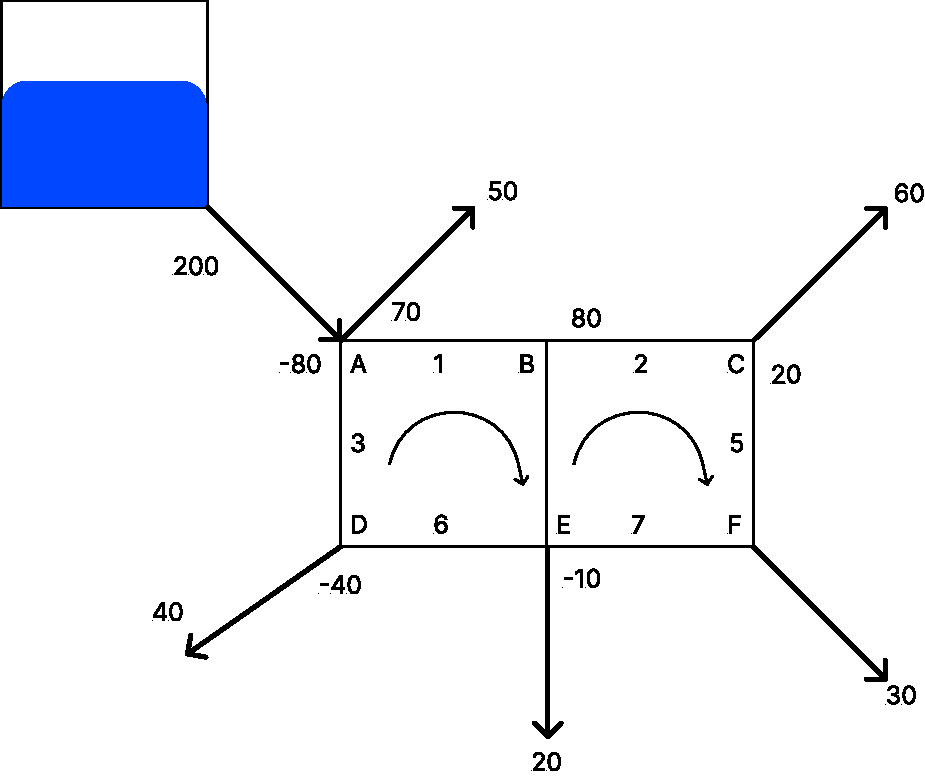
\includegraphics[width=0.5\textwidth]{ha10.pdf}
  \caption{Red cerrada}
  \label{ha10}
\end{figure}
Se separan en dos circuitos y se elaboran dos tablas con los gastos.

\section{Canales}
\subsection{El flujo a superficie libre}
Se define como el flujo a presión atmosférica, de éstos existe el flujo permanente ($\frac{\partial (P,\upsilon) }{\partial \tau}=0$) y no permanente ($\frac{\partial \left(P,\upsilon\right)}{\partial \tau}\neq 0$)

\Schema{-1.4ex}{15ex}
{\schemabox{Flujo a\\Superficie\\Libre}} { \Schema{-1ex}{8ex}
	{\schemabox{Permanente}}
	{
		\schemabox{Uniforme}
		\medskip
		\schema
		{\schemabox{Variado}}
		{\schemabox{Gradualmente\\ Rápidamente\\
				Especialmente}}
	}
	\Schema{-1ex}{5ex}
	{\schemabox{No\\ permanente}}
	{
		\schemabox{Uniforme}
		\medskip
		\schema
		{\schemabox{Variado}}
		{\schemabox{Gradualmente\\ Rápidamente}}}}
	

\begin{figure}[h!]
\centering
  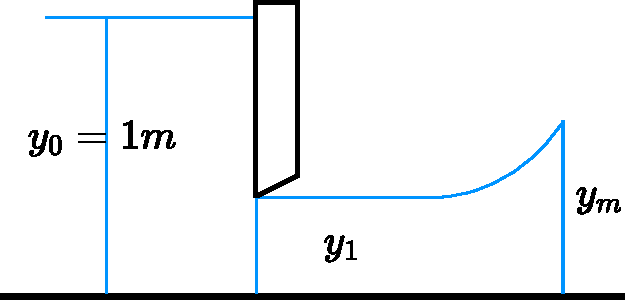
\includegraphics[width=0.5\textwidth]{ha11.pdf}
  \caption{Compuerta con flujo permanente}
  \label{ha11}
\end{figure}
\begin{equation}
    Q = Cd\cdot A \sqrt{2g y_1}
\end{equation}
Analizando el comportamiento, tenemos la siguiente tabla:
\begin{table}[h!]
    \centering
    \begin{tabular}{@{}cc@{}}
    \toprule
    $y_0$ & $\tau$ \\ \midrule
    1m    & 0 seg  \\
    1m    & 10 seg \\
    1m    & 15 seg \\
    1m    & 20 seg \\ \bottomrule
    \end{tabular}
    \caption{Flujo permanente en función del tiempo}
    \label{tabha8}
\end{table}

\begin{example}
    \begin{figure}[h!]
    \centering
      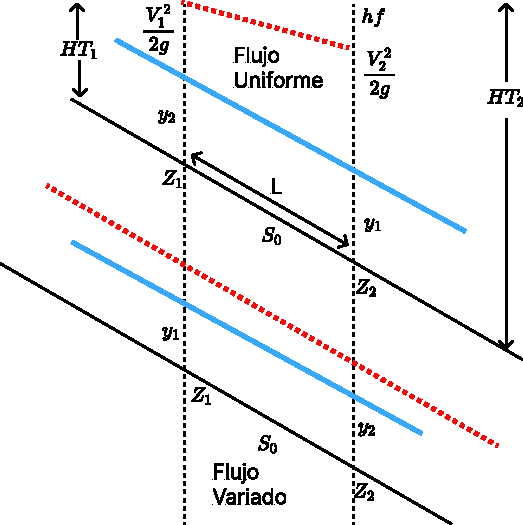
\includegraphics[width=0.5\textwidth]{ha12.pdf}
      \caption{Canal con flujo uniforme (Parte superior) y flujo variado (Parte inferior)}
      \label{ha12}
    \end{figure}
\end{example}

\textit{ Sol. }

Según la figura \ref{ha12}, podemos observar las siguientes propiedades:

\begin{align*}
    \text{Flujo Variado}&&y_1 \neq y_2&& S_0\neq S_f&& S_f\neq S_{\omega}\\
    \text{Flujo Uniforme}&&y_1 = y_2&& S_0 = S_f&&S_0 = S_f = S_{\omega}
\end{align*}

\begin{definition}[Pendient hidráulica]
    \begin{equation}
        S_0 = \frac{\Delta z}{L} = \sin{\left(\frac{\Delta z}{L}\right)} 
    \end{equation}
    Es importante no confundirse con $S_0$ y una pendiente geométrica $m$, puesto que cuando un ángulo $\theta< 10^{\circ}$, entonces $\sin{\theta}\approx \tan{\theta}$
    % $S_{\omega}$ Es la pendiente del agua.
\end{definition}
Recordando las variables que usa el número de Reynolds:
\begin{notation}
    \begin{itemize}
        \item Área hidráulica: $A$
        \item Perímetro Mojado: $P$
        \item Radio Hidráulico: $R_h$
        \item Tirante Hidráulico: $Y\lor D$
    \end{itemize}
\end{notation}

\begin{figure}[h!]
\centering
  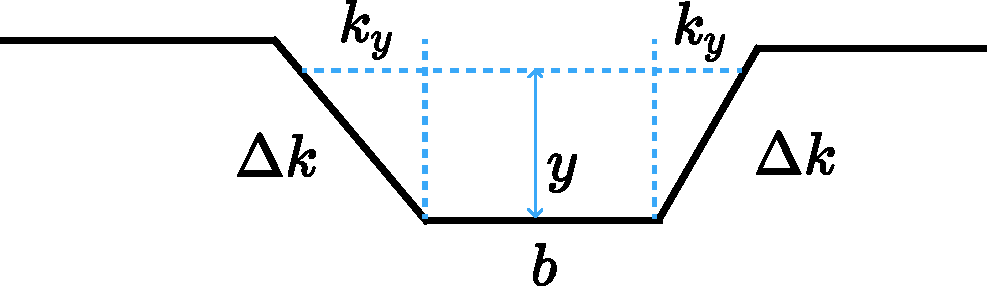
\includegraphics[width=0.5\textwidth]{ha13.pdf}
  \caption{Canal}
  \label{ha13}
\end{figure}

Aplicando un poco de geometría, podemos usar los conceptos anterior mencionados
\begin{align*}
    &A=\left((b + k_1y_1 +k_2y_2) + b \right)\\
    &k_1 = k_2 = k\\
    &A = \left(b + 2ky\right)y\\
    &P = 2 \sqrt{k^2y^2 + y^2} + b\\
    &R_h = \frac{A}{P} =\frac{\left(b + 2ky\right)y}{b +2ky \sqrt{1 +k^2}}\\
\end{align*}
\subsection{Cálculo de flujo uniforme}
\begin{equation}
    \text{Ecuación de Chezy } v= c \sqrt{RS}
\end{equation}
\begin{equation}
    \text{Ecuación de Chezy }Q= \frac{1}{n}R_h^{2/3}S^{1/2}
\end{equation}
Recordando los valores:
\begin{align}
    &A =\left(b + ky\right)y\\
    &P = b + 2y \sqrt{1 +k^2}\\
    &R_h = \frac{A}{P}=\frac{\left(b + ky\right)y}{b + 2y \sqrt{1 +k^2}}\\
    &Q = \frac{1}{n}\cdot \left[\left(b + ky\right)y\right]\cdot \left[\frac{\left(b + ky\right)y}{b + 2y \sqrt{1 +k^2}}\right]^{\frac{2}{3}}\cdot S_0^{\frac{1}{2}}
\end{align}
Por definición el caudal (conocido como gasto $Q=\frac{Volumen}{Tiempo}$) se visualiza como la longitud que pasa a través del tiempo un flujo y se multiplica por su área.
Lo que de otra manera, puede expresarse como la diferencial $dq=\bar{v}\cdot\bar{d}A$, así definimos el caudal como:
\begin{equation}
    Q = \int_a\bar{v}\cdot \bar{a}\,d{A}
\end{equation}

Regresando a la ecuación de Chezy, aplicamos un método numérico.
\subsection{Régimen Crítico}
Planteando la figura \ref{ha14}, se necesita obtener $y_2$ despreciando las pérdidas de energía $h_r=0$.
\begin{figure}[h!]
\centering
  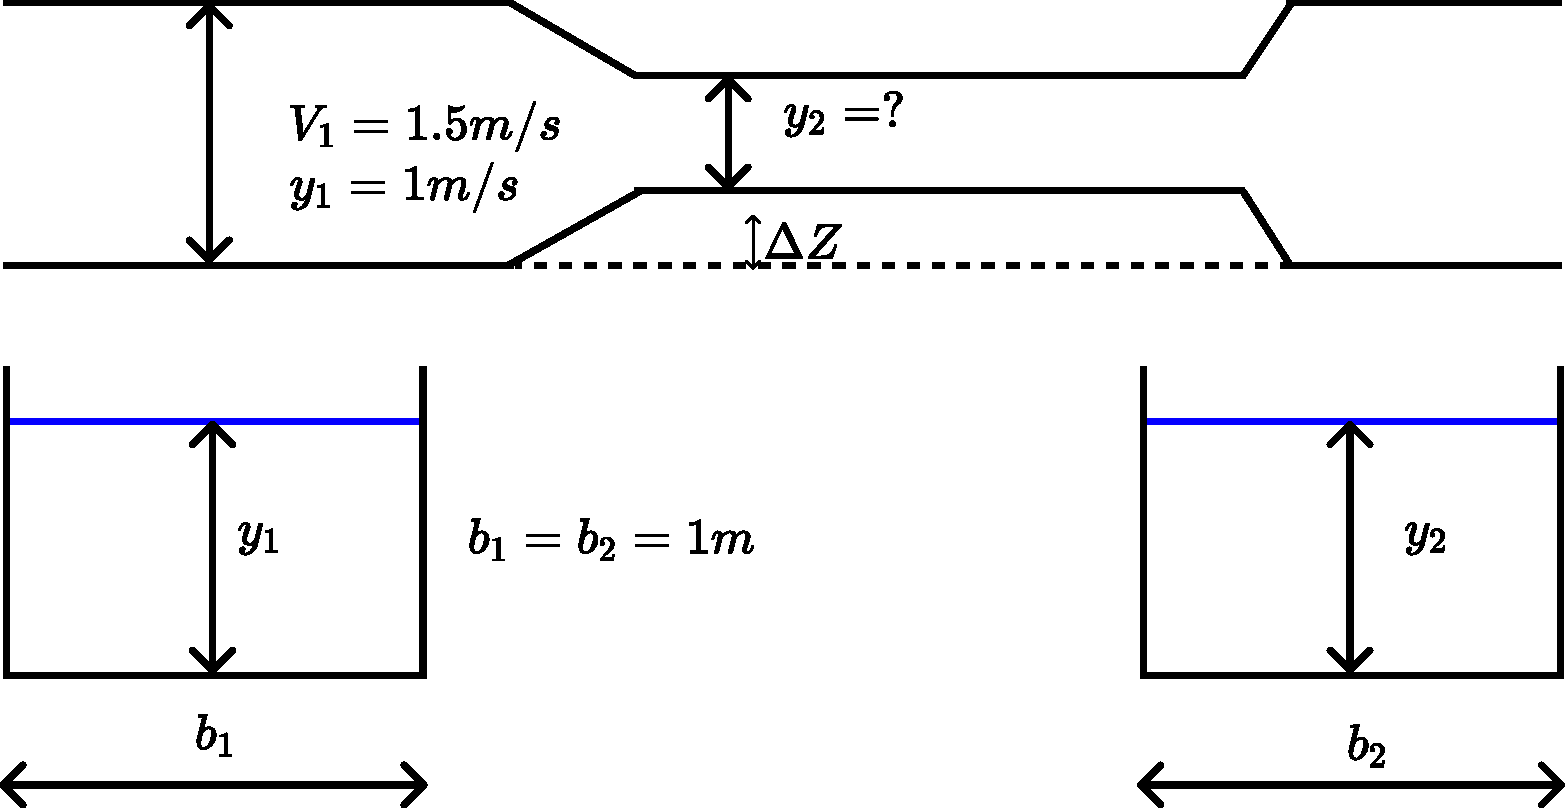
\includegraphics[width=0.5\textwidth]{ha14.pdf}
  \caption{Régimen Crítico}
  \label{ha14}
\end{figure}

\textit{ Sol. }

Podemos expandir mediante la ecuación de Bernoulli que dice
\begin{equation}
    Z_1 +P_1 + \frac{V_1^2}{2g} = Z_2 + P_2 + \frac{V_2^2}{2g} + \sum_1^2hv
\end{equation}
Colocamos las variables en la figura \ref{ha15}:
\begin{figure}[h!]
\centering
  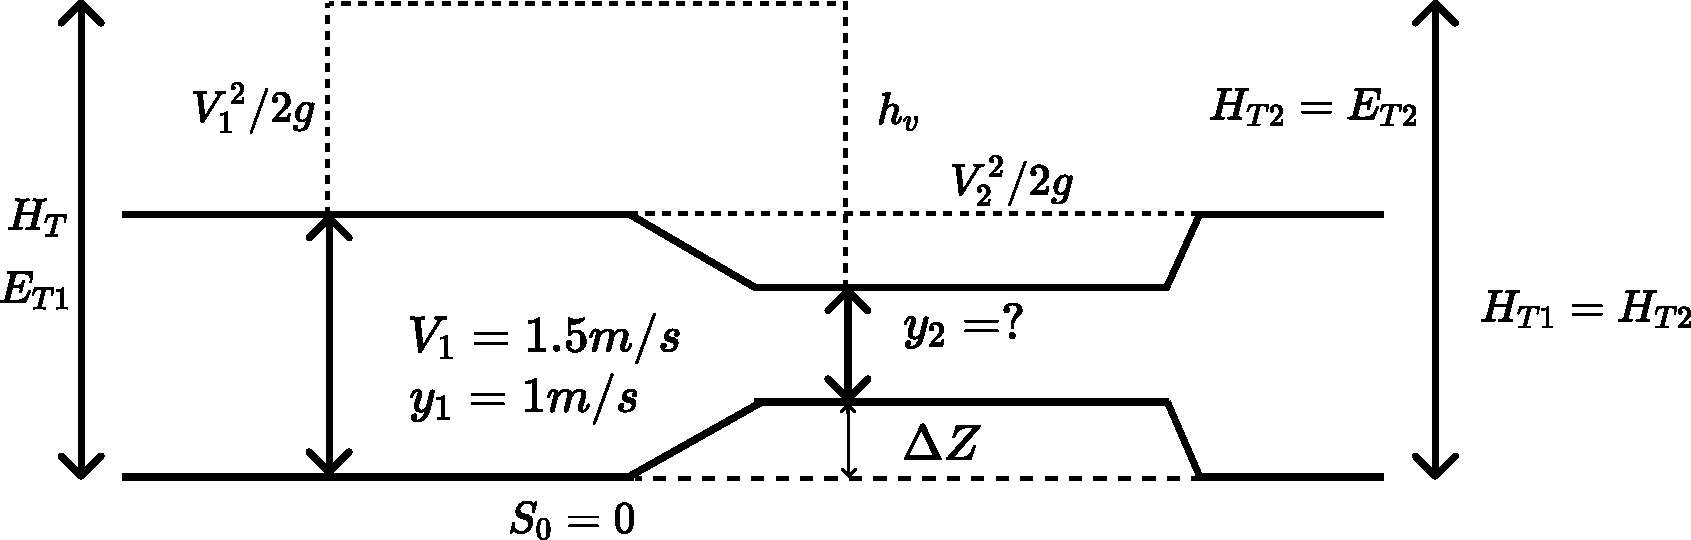
\includegraphics[width=0.5\textwidth]{ha15.pdf}
  \caption{Deducción de la energía específica}
  \label{ha15}
\end{figure}

Ahora sí, podemos definir que la ecuación de la energía específica es:
\begin{align*}
    &E= y + \alpha\cdot \frac{V^2}{2g}\mid\, \alpha =1\\
    &\therefore E= y + \frac{V^2}{2g} = \frac{\text{Energia}}{Peso}\\
    &\implies \frac{E_c = \frac{1}{2}\cdot m\cdot v^2}{Peso = mg}\\
    & \frac{E_p = m \cdot g \cdot z}{M\cdot g}\implies Z
\end{align*}
Despejando variables:
\begin{align*}
    &y_1+ \frac{V_1^2}{2g} = y_2 + \frac{V_2^2}{2g} + h_r+\Delta Z\\
    &y_1 + \frac{V_1^2}{2g} = y_2 + \frac{V_2^2}{2g} +\Delta Z\\
    &E_1 = \Delta Z + E_2\\
    &\therefore \Delta Z = E_1 - E_2
\end{align*}
Sustituyendo los valores de $E_1$ y $E_2$:
\begin{align*}
    y_1+ \underbrace{E_1}{\frac{v_1^2}{2g}} = y_2 + \frac{V_2^2}{2g} +\Delta Z\\
\end{align*}
Como $Q_1=Q_2$ y $V_2=\frac{Q}{A_2}$, se define ahora que $A=b\cdot y$ (Base por altura), y $A_2=b_2\cdot y_2$
\begin{align*}
    &\left(y_1 + \frac{V_1^2}{g_2}\right)\cdot y_2^2 =\Delta z\cdot y_2^2 + y_2^3 + \frac{Q^2}{2gb^2_2}\\
    &y_2^3 +y_2^2\left[\Delta z -\left(y_1 +\frac{V_1^2}{2g} \right) \right] + \frac{Q^2}{2gb_2^2} = 0
\end{align*}
Terminando como:
\begin{equation}
    y_2^3 +y_2^2\left[\Delta z - E_1 \right] + \frac{Q^2}{2gb_2^2} = 0
\end{equation}


\begin{figure}[h!]
\centering
  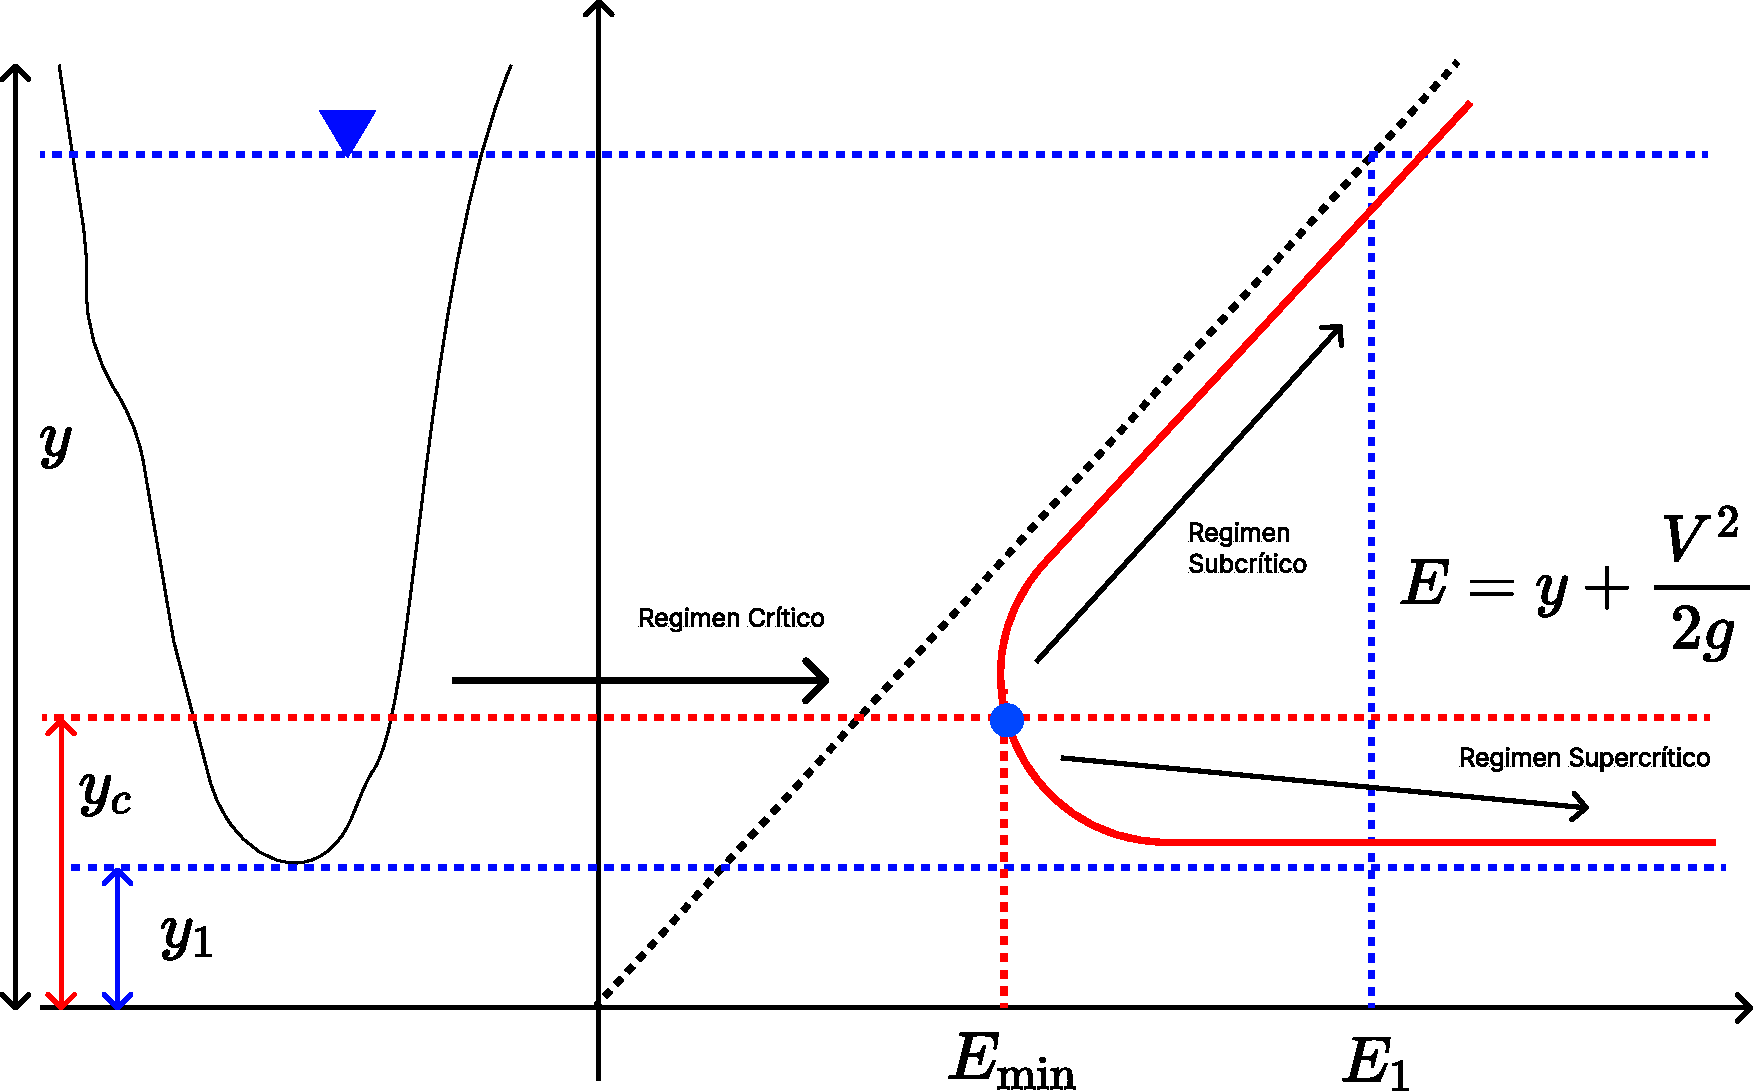
\includegraphics[width=0.5\textwidth]{ha16.pdf}
  \caption{Diferentes tipos de régimenes}
  \label{ha16}
\end{figure}
De manera que se establecen los régimenes como:
\begin{align*}
    y< y_c && \Rightarrow && \text{Subcrítico}\\
    y> y_c && \Rightarrow && \text{Supercrítico}\\
    y= y_c && \Rightarrow && \text{Crítico}
\end{align*}
Recordando que el número de Froude es:
\begin{equation}
    Fr = \frac{v}{\sqrt{g\cdot \frac{A}{T}}} = 1
\end{equation}
Se sabe que $V=Q/A$, así que derivando ésta ecuación obtendríamos:
\begin{align*}
    &\frac{dE}{dy}= \frac{d\left(y + \frac{Q^2}{A^2\cdot 2g}\right)}{dy} = 0\\
    &1 + \frac{Q^2}{2g}\cdot \frac{dA^{ -1}}{dy}= 0\\
    &1 - \frac{Q^2}{g}\cdot \frac{1}{A^3}\cdot \frac{Tdy}{dy}=0\\
    &\therefore \frac{Q^2}{g} = \frac{A^2}{T}\implies y_c\\
    &\frac{Q^2}{g} = \frac{b^3\cdot y^3_c}{b}\\
    &y_c^3 = \frac{Q^2}{b^2}\cdot \frac{1}{g}
\end{align*}

\subsection{Diseño de canales no revestidos}

Son dos los métodos a utilizar:
\begin{itemize}
    \item Método de la velocidad máxima permisible
    \item Método del esfuerzo cortante (Fuerza tractiva)
\end{itemize}

\subsubsection{Método de la velocidad máxima permisible}
\begin{equation}
    V_{\max }\leq V_{permisible}
\end{equation}

El método consiste en fijar una velocidad máxima para evitar erosión y no tan pequeña para evitar no solo sedimentación, sino también el crecimiento de plantas, para ello se utilizan tablas o cuadros de velocidades recomendadas, aunque es muy aventurado se podría considerar un valor del orden de 2.5 pies/seg (Chow 1959), la metodología es la siguiente:

\begin{enumerate}
    \item Para un tipo de material donde se va a diseñar un canal no revestido, estimar el coeficiente de rugosidad ``$n$'' de Manning, inclinación lateral $z=k$ (el valor de $k=1.5$) se ha dado por experiencia y es estable pero conviene revisar tablas disponible (7.1 V.T. Chow o similar), obtener la velocidad permisible $Vp$ si dependiendo del material del canal
    \item Calcular el radio hidráulico con la ecuación de Manning
    \item Calcular el área requerida utilizando el gasto y la velocidad permisible $A= \frac{Q}{Vp}$
    \item Calcular el perimetro mojado $P= \frac{A}{R}$
    \item Con las expresiones de $A$ y $P$ de la tabla 2.1 (Chow , 1959), resolver para b y tirante ``$y$''
    \item Definir el bordo libre BL y modificar la sección para dimensiones prácticas.
\end{enumerate}
\subsection{Flujo gradualmente variado}

\begin{figure}[h!]
\centering
  \includegraphics[width=0.5\textwidth]{ha19.pdf}
  \caption{Flujo en canales, disminución de la pendiente}
  \label{ha19}
\end{figure}
\begin{figure}[h!]
\centering
  \includegraphics[width=0.5\textwidth]{ha20.pdf}
  \caption{Aumento de la pendiente}
  \label{ha20}
\end{figure}

\begin{figure}[h!]
\centering
  \includegraphics[width=0.5\textwidth]{ha21.pdf}
  \caption{Volumen de control diferencial para la derivación de la ecuación dinámica del flujo gradualmente graduado}
  \label{ha21}
\end{figure}
Del principio de conservación de la energía en el volumen diferencial
\begin{equation}
    \frac{\partial H}{\partial S} = \frac{d\left(E = y + \frac{V^2}{2g} \right)}{dx} + \frac{dz}{dx} + \frac{dh_f}{dx} =0
\end{equation}
\begin{notation}
    \begin{itemize}
        \item $H$: Energía total
        \item $S$: Trayectoria
        \item $E$: Energía específica del canal
        \item $y$: tirante vertical
        \item $\frac{dz}{dx}=-S_0$: pendiente del canal
        \item $\frac{dh_f}{dx}=S_f$: pendiente de fricción que para manning es $S_f=\left(Vn/R_h^{2/3}\right)$
    \end{itemize}
\end{notation}
Ecuación que puede simplificarse a:
\begin{equation}
    \frac{dy}{dx} = \frac{S_0 -S_f}{1 - F^2}
\end{equation}
\begin{notation}
    \begin{itemize}
        \item $\frac{dy}{dx}$: variación del tirante a lo largo del canal o dirección ``x''
        \item $S_0$: Pendiente del canal
        \item $S_f$: Pendiente de fricción
        \item $F$: Número adimensional de Froude
    \end{itemize}
\end{notation}
\subsubsection{Clasificación de los perfiles de flujo gradualmente variado permanente}
Descripción de la letra se define por la pendiente del canal $S_0$ , con respecto a la pendiente crítica $S_c$, perfiles suaves (MILD) o letra M: $S_0<S_c$. Existen tres zonas donde se pueden alojar los perfiles:
\begin{itemize}
    \item \textbf{Zona 1}, si el perfil (tirantes) se encuentran por arriba del tirante normal y crítico se conoce como $M_1$
    \item \textbf{Zona 2}, si el perfil (tirantes) se encuentran entre el tirante normal y el crítico, se conoce como $M_2$
    \item \textbf{Zona 3}, si el perfil (tirantes) se encuentran por debajo del tirante crítico y normael se conoce como $M_3$
\end{itemize}

\begin{figure}[h!]
\centering
  \includegraphics[width=0.5\textwidth]{ha22.pdf}
  \caption{Para $M_1: y_c<y_0<y$; $M_2: y_c<y<y_0$;  $M_3: y<y_c<y_0$}
  \label{ha22}
\end{figure}

\begin{figure}[h!]
\centering
  \includegraphics[width=1\textwidth]{ha23.pdf}
  \caption{Tipo de perfiles en flujos de canales abiertos}
  \label{ha23}
\end{figure}

\begin{equation}
    \frac{dy}{dx} = \frac{S_0 -S_f}{1 -F^2_r}
\end{equation}
Con la información y datos del problema en el canal, calcular los tirantes normal, crítico, pendiente crítica y Número de Froude. Clasificar los perfiles que se presentan en el canal. Aplicar la ecuación dinámica y resolverla por cualquier método conocido para encontrar el perfil hidráulico correspondiente

\subsection{Método de integración gráfica}

\begin{align*}
    &\text{Si } \frac{dy}{dx}= \frac{S_0 -S_f}{1 -F^2_r}\\
    &\frac{dx}{dy}= \frac{1 -F^2_r}{S_0 -S_f}\, \text{ Si definimos la función}\\
    &F(y) = \frac{1 -F^2_r}{S_0 -S_f}\implies dx = F(y)\,dy\,\text{ Integrando, entre dos puntos}\\
    &\int_{x1}^{x2}\,dx = \int_{y1}^{y2} F(y)\,dy\,\text{Por teorema fundamental del calculo}\\
    &x_2 -x_1 = \Delta x =\int_{y1}^{y2} F(y)\,dy = F(y)\\
    &\therefore \Delta x= A(y)
\end{align*}
La distancia entre los tierantes $y_1$ e $y_2$ es igual al áera bajo la curva $F(y)$
% Poner una gráfica con A1 +A2=A_T pero no es necesario

\subsubsection{Clasificación de perfiles hidráulicos}

Existe la clasificación por pendiente:

\begin{itemize}
    \item \textbf{Perfiles M}: Pendiente moderada $S_0<S_c$
    \item \textbf{Perfiles S}: Pendiente pronunciada $S_0>S_c$
    \item \textbf{Perfiles H}: Pendiente horizontal $S_0=0$
    \item \textbf{Perfiles C}: Pendiente crítica $S_0=S_c$
    \item \textbf{Perfiles A}: Pendiente adversa o negativa $S_0<0$
\end{itemize}
\begin{figure}[h!]
\centering
\includegraphics[width=0.5\textwidth]{ha17.pdf}
\caption{Clasificación por zonas, pendiente moderada, pendiente pronunciada, pendiente horizontal, pendiente crítica y pendiente adversa}
\label{ha17}
\end{figure}
\begin{figure}[h!]
    \centering
    \includegraphics[width=0.5\textwidth]{ha18.pdf}
    \caption{Clasificación por zonas, pendiente pronunciadas}
    \label{ha18}
\end{figure}

\begin{example}
    Un canal de sección trapecial, ancho de plantilla de 8m y taludes 1:5;1 está excavado en tierra (Coeficiente de Manning $n=0.025$) con una pendiente de plantilla $S_0=0.0009$ y debe conducir un gasto de $15m^3/s$ figura \ref{ha24}. Con objeto de dar carga sobre una serie de orificios laterales, se utiliza un cimacio vertedor con longitud de cresta $b=12m$. La let de gastos de vertido sobre el mismo es $Q=2bh^{3/2}$ y la altura de la cresta al fondo es $2=1.77m$
\end{example}
\begin{figure}[h!]
\centering
  \includegraphics[width=0.5\textwidth]{ha24.pdf}
  \caption{Canal de ejemplo}
  \label{ha24}
\end{figure}

\textit{ Sol. }

Para el cálculo de tirante normal y crítico; el tirante normal $y_0$ con la ecuación de Manning y con el método de aproximaciones:
\begin{align*}
    A\cdot R_h^{\frac{2}{3}} = \frac{nQ}{\sqrt{S}}\\
    y_0 = 1.265m
\end{align*}
Tirante crítico, $yc$ con la ecuación Energía específica mínima, por el método de aproximaciones
\begin{align*}
    &\frac{Q^2}{\frac{g}{\alpha}} = \frac{A_c^3}{T_c}\\
    &y_c = 0.678m
\end{align*}
Calculando la pendiente crítica con la ecuación 
\begin{equation*}
    S_f = \left(\frac{V\cdot n}{R_h^{\frac{2}{3}}}\right)
\end{equation*}
Resulta $S_0<S_c$ además $y_c<y_0<y$, Entonce se clasifica como $M_1$

Los límites de Integración, son las secciones de control y se encuentran en todo punto donde haya una relación Gasto-Carga, Por ejemplo: Vertedores, compuertas, tirante normal y el tirante crítico\footnote{Cuando se utilice el tirante normal y tirante crítico como límites de integración, se toma el límite con un pequeño porcentaje de los tirantes anteriores, por ejemplo 1 al 3\% de error dependiendo de la zona. El perfil nunca puede cruzar de una zona a otra, ejemplo el $M$ no pasa el cálculo del perfil de la Zona 1 a la Zona 2 o a la Zona 3.}

\begin{example}
    $Q=15 m^3/s,\, k=1.5,\, b=8m,\, S_0u= 0.000$ una presa derivadora que tiene un vertedor de altura y longitud de cresta de $w=1.77m, 12m$
\end{example}
\textit{ Sol. }
\begin{align*}
    Q = 2bh^{3/2}\\
    h = \left(\frac{Q}{2b}\right)^{\frac{2}{3}}\\
    \left(\frac{15}{24}\right)^{\frac{2}{3}} = 0.731m\\
    \Delta x =\int_{y1}^{y2}F(y)\,dy
\end{align*}
\begin{figure}[h!]
\centering
  \includegraphics[width=0.5\textwidth]{ha25.pdf}
  \caption{Área bajo la curva de la función $F(y)$}
  \label{ha25}
\end{figure}
\begin{align*}
    &F(y) = \frac{1 - F_r^2}{S_0 - S_f}&& S_f =\left(\frac{Vn}{R_h^{\frac{2}{3}}}\right)^2&&Fr = \frac{v}{\sqrt{g\cdot \frac{A}{T}}}\\
    &V =\frac{Q}{A}&&R_h = \frac{A}{P}&&A =(b+ ky)\cdot y\\
    &P = b + 2ky \sqrt{1 + k^2}&& T =b + 2ky&&F(y) = \frac{1 -F^2_r}{S_0 -S_f}
\end{align*}


\subsection{Método de incrementos finitos}
Cuando se aplicó la ecuación de energía (Bernoulli), en el volumen de control con distancia $dx$ se obtuvo la ecuación:
\begin{equation*}
    \frac{dE}{dx} - S_0 + S_f =0\quad \lor\quad \frac{dE}{dx} =S_0 - S_f
\end{equation*}
Si se invierte a su recíproco:
\begin{equation*}
    \frac{dx}{dE} = \frac{1}{S_0 - S_f}\implies dx = \frac{dE}{S_0 - S_f}
\end{equation*}
En incrementos finitos:
\begin{equation}
    \Delta x = \frac{\Delta}{S_0 -\bar{S}_f}
\end{equation}
Donde:
\begin{align*}
    &\Delta E = E_1 - E_2\\
    &E_1 = y_1 + \frac{V_1^2}{2g}\\
    &E_2 = y_2 + \frac{V_2^2}{2g}\\
    &S_f = \frac{Sf_1+ Sf_2}{2}\\
    &S_f = \frac{v^2n^2}{R^{\frac{4}{3}}}\\
    &\bar{v} = \frac{Q}{A}\quad R = \frac{A}{P}
\end{align*}

\begin{definition}[Salto hidráulico]
    Es el cambio de un flujo supercrítico a subcrítico, en flujo rápidamente variado.
\end{definition}

\begin{figure}[h!]
\centering
  \includegraphics[width=0.5\textwidth]{ha27.pdf}
  \caption{Salto hidráulico}
  \label{ha27}
\end{figure}

\begin{figure}[h!]
    \centering
      \includegraphics[width=0.5\textwidth]{ha29.pdf}
      \caption{Salto ahogado}
      \label{ha29}
\end{figure}
En la figura \ref{ha29}, el agua lo empuja y se ahoga la velocidad.

\begin{figure}[h!]
\centering
  \includegraphics[width=0.5\textwidth]{ha30.pdf}
  \caption{Salto Barrido}
  \label{ha30}
\end{figure}

\begin{figure}[h!]
\centering
  \includegraphics[width=0.5\textwidth]{ha31.pdf}
  \caption{Segundo ejemplo de un salto Barrido}
  \label{ha31}
\end{figure}

\begin{figure}[h!]
\centering
  \includegraphics[width=0.5\textwidth]{ha32.pdf}
  \caption{Cálculo del salto hidráulico}
  \label{ha32}
\end{figure}

\begin{figure}[h!]
\centering
  \includegraphics[width=0.5\textwidth]{ha33.pdf}
  \caption{Entre perfiles S2 y S1}
  \label{ha33}
\end{figure}

\begin{figure}[h!]
\centering
  \includegraphics[width=0.5\textwidth]{ha34.pdf}
  \caption{Entre perfiles S3 y S1}
  \label{ha34}
\end{figure}

% \begin{figure}[h!]
%     \centering
%       \includegraphics[width=0.5\textwidth]{ha35.pdf}
%       \caption{Entre perfiles M3 y M1}
%       \label{ha35}
%     \end{figure}

\begin{figure}[h!]
\centering
  \includegraphics[width=0.5\textwidth]{ha35.pdf}
  \caption{Cambio brusco de pendiente}
  \label{ha35}
\end{figure}

\begin{figure}[h!]
\centering
  \includegraphics[width=0.5\textwidth]{ha36.pdf}
  \caption{Flujo uniforme}
  \label{ha36}
\end{figure}

\begin{figure}[h!]
\centering
  \includegraphics[width=0.5\textwidth]{ha37.pdf}
  \caption{Integración de los perfiles hidráulicos: Disminución de la pendiente}
  \label{ha37}
\end{figure}

\begin{figure}[h!]
\centering
  \includegraphics[width=0.5\textwidth]{ha38.pdf}
  \caption{Aumento de la pendiente}
  \label{ha38}
\end{figure}
\section{Aforadores en Canales}
Un canal sin aforar no es útil, existen muchos tipos de aforadores. Antiguamente se usaba el canal tipo Parshall (Dos tomas),
pero existía el problema de que se hundía. El vertedor de cresta ancha ``aforador de garganta'' es auto-calibrable, softwares para diseñar, para ésta Sección
sólo importa usar el programa HCanales para diseñar. Consiste en el canal que se obtenga el tirante crítico para calcular el gasto.

\subsection{Sedimentación y erosión en canales}

En los canales artificiales, existen tanques de sedimentación que disminuye la velocidad para depositar los sedimentos.

La velocidad máxima permisible sirve para diseñar canales no revestidos, véase la tabla siguiente:
\begin{table}[h!]
    \centering
    \begin{tabular}{@{}ccc@{}}
    \toprule
    Autor &
      Ecuación &
      Comentarios \\ \midrule
    \begin{tabular}[c]{@{}c@{}}Lischtvan-Levediev\\ (1959)\end{tabular} &
      \begin{tabular}[c]{@{}c@{}}$\frac{V_c}{\sqrt{(S_s-1)g\cdot d}}=1.63\left(\frac{y}{d}\right)^{0.1283}$ Para $\frac{y}{d}\leq 744.19$\\ $\frac{V_c}{\sqrt{(S_s-1)g\cdot d}}=1.4527\left(\frac{y}{d}\right)^{0.3221}$ Para $\frac{y}{d}> 744.19$\end{tabular} &
      \begin{tabular}[c]{@{}c@{}}$d$ diámetro medio de las\\ partículas en $m$,\\ $y$ tirante en $m$,\\ $S_s$ densidad relativa del material\\ (Ecuaciones de ajuste según García\\ Flores)\end{tabular} \\
    Goncharov (1964) &
      \begin{tabular}[c]{@{}c@{}}$\frac{V_c}{\sqrt{(S_s-1)g\cdot d}}=1.069\log{\left(8.8\frac{y}{d}\right)}$\\ $\frac{V_c}{\sqrt{(S_s-1)g\cdot d}}=0.75593\log{\left(8.8\frac{y}{d}\right)}$\end{tabular} &
      \begin{tabular}[c]{@{}c@{}}$V_s$ velocidad de separación;\\ $V_c$ velocidad permisible (Sin separación).\\ Se relacionan mediane la expresión\\ $V_s=1.41421\cdot V_p$\\ $d$ diámetro medio de las partículas cuan-\\ do la granulometría no es uniforme.\end{tabular} \\
    Maza-García (1978) &
      $\frac{V_c}{\sqrt{(S_s-1)g\cdot d}}=1.504\left(\frac{y}{d}\right)^{0.15}$ &
      \begin{tabular}[c]{@{}c@{}}$V_c$ velocidad crítica media, $d$ el diámetro $d_m$\\ cuando la granulometría no es uniforme.\\ Pared hidráulicamente rugosa.\end{tabular} \\
    Neill (1968) &
      $\frac{V_c}{\sqrt{(S_s-1)g\cdot d}}=1.414\left(\frac{y}{d}\right)^{1/6}$ &
      \begin{tabular}[c]{@{}c@{}}$V_c$ velocidad crítica media.\\ Pared hidráulicamente rugosa.\\ $d$ diámetro medio de las partículas\end{tabular} \\
    Garde (1970) &
      $\frac{V_c}{\sqrt{(S_s-1)g\cdot d}}=0.5\log{\left(frac{y}{d}\right)}+1.63$ &
      \begin{tabular}[c]{@{}c@{}}$V_c$ velocidad crítica media.\\ Pared hidráulicamente rugosa.\\ $d$ diámetro medio.\end{tabular} \\
    Levi &
      \begin{tabular}[c]{@{}c@{}}$\frac{V_c}{\sqrt{g\cdot d_m}}=1.4\left[1+\ln{\left(\frac{y}{7\cdot d_m}\right)^{1/2}}\right]\cdot \left(\frac{d_{max}}{d_m}\right)^{1/7}$ Para $10<\frac{y}{d_m}<60$\\ $\frac{V_c}{\sqrt{g\cdot d_m}}=1.4\left[\frac{d_{max}}{d_m}\right]^{1/7}\cdot \ln{\left(\frac{y}{7\cdot d_m}\right)}$ Para $\frac{y}{d_m}>60$\end{tabular} &
      \begin{tabular}[c]{@{}c@{}}$d_m$ y $d_{so}$ son diámetros característicos del\\ material. Cuando es uniforme $d_{max}=d_m$\\ $V_c$ velocidad crítica media.\\ Pared hidráulicamente rugosa.\end{tabular} \\ \bottomrule
    \end{tabular}
    \caption{Velocidad máxima permisible $V_c$ (no erosiva) en canales con suelos no cohesivos, según distintos autores (García Flores y Maza,1996)}
    \label{tabha9}
\end{table}
\begin{table}[h!]\centering
    \begin{tabular}{@{}ccc@{}}
    \toprule
    Autor        & Ecuación                                               & Comentarios                                                                           \\ \midrule
    \begin{tabular}[c]{@{}c@{}}Mavis-Laushey\\ (1949)\end{tabular} &
      $v_{bc}=0.152d^{4/9}\cdot\left(S_s-1\right)^{1/2}$ &
      \begin{tabular}[c]{@{}c@{}}$d$ diámetro caracterís-\\ tico del material en\\ mm y $v_{bc}$ en m/s\end{tabular} \\
    Carstens (1966) &
      $\frac{v_{bc}}{\sqrt{\left(s_s-1\right)g\cdot d}}=\left[3.61\left(\tan{\gamma}\cos{\theta}-\sin{\theta}\right)\right]^{1/2}$ &
      \begin{tabular}[c]{@{}c@{}}$\gamma$ ángulo de reposo\\ del sedimento y $\theta$\\ ángulo que forma el\\ lecho con la hori-\\ zontal (en dirección\\ longitudinal).\end{tabular} \\
    Garde (1970) & $\frac{v_{bc}}{\sqrt{\left(s_s-1\right)g\cdot d}}=1.51$ & \begin{tabular}[c]{@{}c@{}}$d$ diámetro caracterís-\\ tico del material.\end{tabular} \\
    \begin{tabular}[c]{@{}c@{}}Maza y García Flores\\ (1985)\end{tabular} &
      $\frac{v_{bc}}{\sqrt{\left(s_s-1\right)g\cdot d}}=1.11\left(\frac{y}{d}\right)^{0.05}$ &
      \begin{tabular}[c]{@{}c@{}}$y$ tirante el flujo,\\ $d$ diámetro medio\\ cuando el material no\\ es uniforme.\end{tabular} \\ \bottomrule
    \end{tabular}
    \caption{Velocidad crítica cerca del fondo (no erosiva) en canales ocn suelos no cohesivos, según distintos autores (García Flores y Maza, 1996)}
    \label{tabha10}
\end{table}
\begin{table}[h!]\centering
    \begin{tabular}{@{}|l|ll|llllllllllllllll|@{}}
    \toprule
    \multirow{3}{*}{\begin{tabular}[c]{@{}l@{}}Denominación de los\\ suelo\end{tabular}} &
      \multicolumn{2}{l|}{\multirow{2}{*}{\begin{tabular}[c]{@{}l@{}}Diámetro medio (en\\ mm) y porcentaje del\\ contenido de partículas\end{tabular}}} &
      \multicolumn{4}{l|}{\begin{tabular}[c]{@{}l@{}}Suelos poco compactos,\\ con densidad relativa del\\ material seco hasta 1.2\\ relación de vacíos mayor\\ de 1.2\end{tabular}} &
      \multicolumn{4}{l|}{\begin{tabular}[c]{@{}l@{}}Suelos medianamente\\ compactos, con densidad\\ relativa del material seco\\ de 1.2 a 1.66, relación\\ de vacíos de 1.2 a 0.6\end{tabular}} &
      \multicolumn{4}{l|}{\begin{tabular}[c]{@{}l@{}}Suelos compactos,\\ con densidad relativa\\ del material seco de\\ 1.66 a 2.04, relación\\ de vacíos de 0.6 a\\ 0.3\end{tabular}} &
      \multicolumn{4}{l|}{\begin{tabular}[c]{@{}l@{}}Suelos muy compactos,\\ con densidad relativa\\ del material seco de\\ 2.04 a 2.14, relación\\ de vacíos de 0.3 a 0.2\end{tabular}} \\ \cmidrule(l){4-19} 
     &
      \multicolumn{2}{l|}{} &
      \multicolumn{16}{l|}{Tirante en m} \\ \cmidrule(l){2-19} 
     &
      \multicolumn{1}{l|}{\begin{tabular}[c]{@{}l@{}}<0.005\\ (mm)\end{tabular}} &
      \begin{tabular}[c]{@{}l@{}}0.005 a 0.05\\ (mm)\end{tabular} &
      \multicolumn{1}{l|}{0.4} &
      \multicolumn{1}{l|}{1.0} &
      \multicolumn{1}{l|}{2.0} &
      \multicolumn{1}{l|}{\begin{tabular}[c]{@{}l@{}}3.0\\ o\\ más\end{tabular}} &
      \multicolumn{1}{l|}{0.4} &
      \multicolumn{1}{l|}{1.0} &
      \multicolumn{1}{l|}{2.0} &
      \multicolumn{1}{l|}{\begin{tabular}[c]{@{}l@{}}3.0\\ o\\ más\end{tabular}} &
      \multicolumn{1}{l|}{0.4} &
      \multicolumn{1}{l|}{1.0} &
      \multicolumn{1}{l|}{2.0} &
      \multicolumn{1}{l|}{\begin{tabular}[c]{@{}l@{}}3.0\\ o\\ más\end{tabular}} &
      \multicolumn{1}{l|}{0.4} &
      \multicolumn{1}{l|}{1.0} &
      \multicolumn{1}{l|}{2.0} &
      \begin{tabular}[c]{@{}l@{}}3.0\\ o\\ más\end{tabular} \\ \midrule
    \begin{tabular}[c]{@{}l@{}}Arcillas\\ Suelos muy arcillosos\\ Suelos poco arcillosos\end{tabular} &
      \multicolumn{1}{l|}{\begin{tabular}[c]{@{}l@{}}30 a 50\%\\ 20 a 30\%\\ 10 a 20\%\end{tabular}} &
      \begin{tabular}[c]{@{}l@{}}50 a 70\%\\ 70 a 80\%\\ 80 a 90\%\end{tabular} &
      \multicolumn{1}{l|}{0.35} &
      \multicolumn{1}{l|}{0.4} &
      \multicolumn{1}{l|}{0.46} &
      \multicolumn{1}{l|}{0.50} &
      \multicolumn{1}{l|}{0.7} &
      \multicolumn{1}{l|}{0.85} &
      \multicolumn{1}{l|}{0.95} &
      \multicolumn{1}{l|}{1.1} &
      \multicolumn{1}{l|}{1.0} &
      \multicolumn{1}{l|}{1.2} &
      \multicolumn{1}{l|}{1.4} &
      \multicolumn{1}{l|}{1.5} &
      \multicolumn{1}{l|}{1.4} &
      \multicolumn{1}{l|}{1.7} &
      \multicolumn{1}{l|}{1.9} &
      2.1 \\ \midrule
    \begin{tabular}[c]{@{}l@{}}Suelos de aluvión,\\ arcillas margosas\end{tabular} &
      \multicolumn{1}{l|}{} &
       &
      \multicolumn{1}{l|}{0.27} &
      \multicolumn{1}{l|}{0.32} &
      \multicolumn{1}{l|}{0.37} &
      \multicolumn{1}{l|}{0.40} &
      \multicolumn{1}{l|}{0.6} &
      \multicolumn{1}{l|}{0.7} &
      \multicolumn{1}{l|}{0.8} &
      \multicolumn{1}{l|}{0.85} &
      \multicolumn{1}{l|}{0.8} &
      \multicolumn{1}{l|}{1.0} &
      \multicolumn{1}{l|}{1.2} &
      \multicolumn{1}{l|}{1.3} &
      \multicolumn{1}{l|}{1.1} &
      \multicolumn{1}{l|}{1.3} &
      \multicolumn{1}{l|}{1.5} &
      1.7 \\ \midrule
    Suelos arenosos &
      \multicolumn{1}{l|}{5 a 10\%} &
      20 a 40\% &
      \multicolumn{16}{l|}{De acuerdo con el tamaño de las fracciones arenosas} \\ \bottomrule
    \end{tabular}
    \caption{Velocidad media permisible (no erosivas) en m/s para suelos cohesivos en canales rectos, según Lischtvan-Levediev (1959)}
    \label{tabha11}
\end{table}
























































